\documentclass[10pt,onecolumn]{IEEEtran}
\usepackage{fontspec}
\setmainfont{Times New Roman}
\setmonofont{Times New Roman}
\usepackage{amsmath,amssymb,amsthm}
\usepackage{booktabs,array,graphicx,longtable}
\usepackage[hidelinks]{hyperref}
\renewcommand{\thesection}{S\arabic{section}}
\renewcommand{\thesubsection}{\thesection.\arabic{subsection}}
\renewcommand{\thetable}{S\arabic{table}}
\renewcommand{\thefigure}{S\arabic{figure}}
\renewcommand{\theequation}{S\arabic{equation}}
\makeatletter
\newenvironment{suppnonfloattable}{\par\noindent\begin{minipage}{\textwidth}\centering\def\@captype{table}}{\end{minipage}\par}
\makeatother
\setlength{\emergencystretch}{2em}

\begin{document}
\title{Supplementary Evidence for\\
RAAH-ZT: Risk-Aware Adaptive Hysteresis\\
for Stable Zero-Trust Access Control in IoT Networks}
\author{Lei Shu, Weijie Tan, Zhi Ouyang, Kun Niu, Xiuzhang Yang, and Yuling Chen}
\maketitle

\noindent\textbf{Evidence status.}
This supplement documents corrected analysis, a newly implemented
exploratory replay, and retained reconstruction evidence for the
original three-action stabilization question. Source-IP histories
scope the temporal proxy study; separate scripted gateway cases
check factor completion and resource delivery. Section S6 records
the reconstruction provenance, and Section S7 contains all results added in the
first revision (IoT-76550-2026).

\section{Theory and correction ledger}
\label{sec:supp_theory}

\subsection{Adjacent decisions and the active boundary}
For independent, identically distributed Gaussian errors
\(\varepsilon_{t-1},\varepsilon_t\) with standard deviation
\(\sigma>0\), let \(D_k=\mathbf1\{m+\varepsilon_k>\theta\}\) and
\(p=\Phi((m-\theta)/\sigma)\). The two disjoint switch events give
\[
 \Pr(D_t\ne D_{t-1})=2p(1-p)\le\tfrac12 .
\]
At \(m=\theta\), both the one-epoch high-decision probability
and the adjacent switch probability are \(1/2\). The submitted
formula \(2\Phi(-|m-\theta|/\sigma)\), which gives one at that
point, is withdrawn. With independent unequal marginal
probabilities \(p_{t-1},p_t\), the probability instead is
\(p_{t-1}(1-p_t)+(1-p_{t-1})p_t\); correlated errors require
their joint law. These statements concern a binary comparison,
not the fused Deny/MFA/Allow action.

For fixed \(\theta_{\rm low}<\theta_{\rm high}\), the active
boundary is \(\theta_{\rm low}\) when the previous internal
state is High and \(\theta_{\rm high}\) when it is Low. With
latent score \(m\), the noisy and unperturbed state updates
agree whenever \(|\varepsilon_t|\) is strictly smaller than
the positive distance from \(m\) to that active boundary.
The proof is the strict comparison defining each transition:
noise shorter than the applicable distance cannot reverse it.
Within the dead zone the margins are
\(m-\theta_{\rm low}\) from High and
\(\theta_{\rm high}-m\) from Low; both equal
\(\Delta/2\), \(\Delta=\theta_{\rm high}-\theta_{\rm low}\),
only at the midpoint. There is no positive uniform margin
for latent scores arbitrarily close to a boundary. This
replaces the submitted unconditional \(\Delta/2\) guarantee.
For \(m\) inside the dead zone and independent
\(\mathcal N(0,\sigma^2)\) error, the one-step state-change
probabilities are respectively
\(Q((m-\theta_{\rm low})/\sigma)\) from High and
\(Q((\theta_{\rm high}-m)/\sigma)\) from Low,
where \(Q=1-\Phi\). These are one-step internal-state
probabilities; final-action SR is reported separately.

\subsection{Finite sampled variation}
For fixed thresholds and observed samples \(x_0,\ldots,x_n\),
let \(K_h(n)=\sum_{t=1}^n\mathbf1\{S_t\ne S_{t-1}\}\) and
\(V_n=\sum_{t=1}^n|x_t-x_{t-1}|\). Then
\[
 K_h(n)\le1+V_n/\Delta. \tag{S1}
\]
Successive binary-state switches alternate direction and their
observed scores lie beyond opposite thresholds. Each disjoint
between-switch interval therefore contributes more than
\(\Delta\) of sampled variation; the cases of zero or one
switch are immediate. This result concerns a fixed-threshold
internal state. An adaptive controller can change active
versions between separately evolved shadow states; that
version edge still counts in final-action SR. The submitted
Brownian exponential ratio and five-order switching claim
do not follow and are withdrawn.

\subsection{Conservative fusion and disposition}
The internal High state is neither authentication nor
entitlement. Deny and pending MFA are preserved in either
state; only a preliminary Allow may become pending MFA
when the state is Low. A verifier result returns to an
independent current guard. The original figure's cell
showing Low state with high risk as Allow contradicted
the source fusion table and is not reused.
\begin{table}[!htbp]
\centering
\caption{Corrected fusion. MFA remains a pending challenge, not a grant.}
\label{tab:supp_fusion}
\footnotesize
\begin{tabular}{lcc}
\toprule
Evaluator output & High internal state & Low internal state\\
\midrule
Deny & Deny & Deny\\
MFA & MFA & MFA\\
Allow & Allow & MFA\\
\bottomrule
\end{tabular}
\end{table}
\begin{table}[!htbp]
\centering
\caption{Treatment of the submitted analytic and reporting claims.
The treatments do not retrospectively verify missing original tables.}
\label{tab:supp_corrections}
\footnotesize
\begin{tabular}{p{.27\textwidth}p{.62\textwidth}}
\toprule
Submitted issue & Revision disposition\\
\midrule
Flip probability one at threshold & Corrected to \(2p(1-p)=1/2\) under independent identical threshold observations.\\
Uniform half-width noise guarantee & Replaced by distance to the active threshold; midpoint is a special case.\\
Brownian exponential ratio and five-order claim & Withdrawn; only the conditional sampled internal-state variation bound remains.\\
BO regret and 20--50-iteration optimality & Withdrawn; finite-budget GP-LCB is reported as a heuristic with full shadow computation.\\
High-state Deny/MFA promotion & Removed; neither hard Deny nor pending MFA can be lifted by state memory.\\
Always-MFA accuracy and ten-pair \(p<0.001\) & Old interpretations withdrawn; class-specific MFA, strict accuracy and descriptive proxy intervals replace them.\\
Submillisecond path and universal evaluator benefit & Withdrawn; S5 separates arithmetic from end-to-end time and S2--S3 retain failures.\\
\bottomrule
\end{tabular}
\end{table}
\section{Data, fitting, and retained reconstruction evidence}
\label{sec:supp_data}

\subsection{Chronological HGB provenance}
After removal of three raw-shard boundary duplicates, the
UNSW-NB15 reconstruction~\cite{unsw_nb15} contains 2,540,044 flows.
A frozen time boundary allocates 1,270,024 records to
early training, 508,020 to validation and 762,000 to test
(613,448 benign and 148,552 attack-labeled test flows).
HGB is fitted on a newly seeded balanced 50,000-row subset
of early training. The first chronological validation half
(254,067 records, including tied boundary seconds) fits
sigmoid calibration, and the later portion selects policy
parameters. The boundary-purged compact input of the new
controller comparison has 253,933 validation events.
Training-only transformations include median imputation,
scaling, clipping to \([-10,10]\), and categorical encoding.
The recorded feature specification contains 40 numeric
and three categorical fields. IPs, timestamps, attack names
and labels are excluded from the model feature matrix.

The centroid trust input uses benign training data and
the training-distance 99th percentile before clipping to
\([0,100]\); the empirical test score has no added artificial
noise. A classifier-derived alternative uses
\(100(1-\widehat p_{\rm attack})\).
These scores are constructed flow diagnostics, not identity
assurance. The test includes 40 source-IP proxies, 38 of
which have adjacent records. There are 761,960 eligible
within-proxy edges; 576,912 connect records with the same
recorded second. Within a proxy, the primary order is
start second then original row ID. Controllers start Low
and reset at validation/test boundaries, with no inferred
within-period inactivity reset. Replay begins after
complete-flow features have been materialized.

\subsection{Retained evaluator and score-source observations}
\begin{table}[!htbp]
\centering
\caption{Retained exploratory chronological UNSW-NB15 source-IP-proxy comparisons from the earlier reconstruction (percent). Hyst is validation-selected BO hysteresis; SMA received the same 50-candidate tuning budget. These rounded results are not recovered original-submission numbers. Benign MFA is a pending challenge, not a completed access result.}
\label{tab:supp_retained_evaluators}
\scriptsize
\setlength{\tabcolsep}{3pt}
\begin{tabular}{llrrrrr}
\toprule
Evaluator & Score & Base SR & Hyst SR & SMA SR & Hyst MFA$_b$ & Hyst FAR$_d$\\
\midrule
RF & Centroid & 0.40 & 1.76 & 0.44 & 12.67 & 0.037 \\
RF & Classifier & 0.40 & 0.40 & 0.40 & 0.02 & 0.037 \\
HGB & Centroid & 2.10 & 3.50 & 2.14 & 7.21 & 0.917 \\
HGB & Classifier & 2.10 & 1.82 & 1.72 & 1.35 & 0.092 \\
LR & Centroid & 1.58 & 2.98 & 1.62 & 6.93 & 0.391 \\
LR & Classifier & 1.58 & 1.54 & 1.47 & 0.67 & 0.199 \\
MLP & Centroid & 0.97 & 2.30 & 1.00 & 12.89 & 0.526 \\
MLP & Classifier & 0.97 & 0.94 & 0.89 & 0.29 & 0.321 \\
\bottomrule
\end{tabular}
\end{table}

\begin{figure}[!t]
\centering
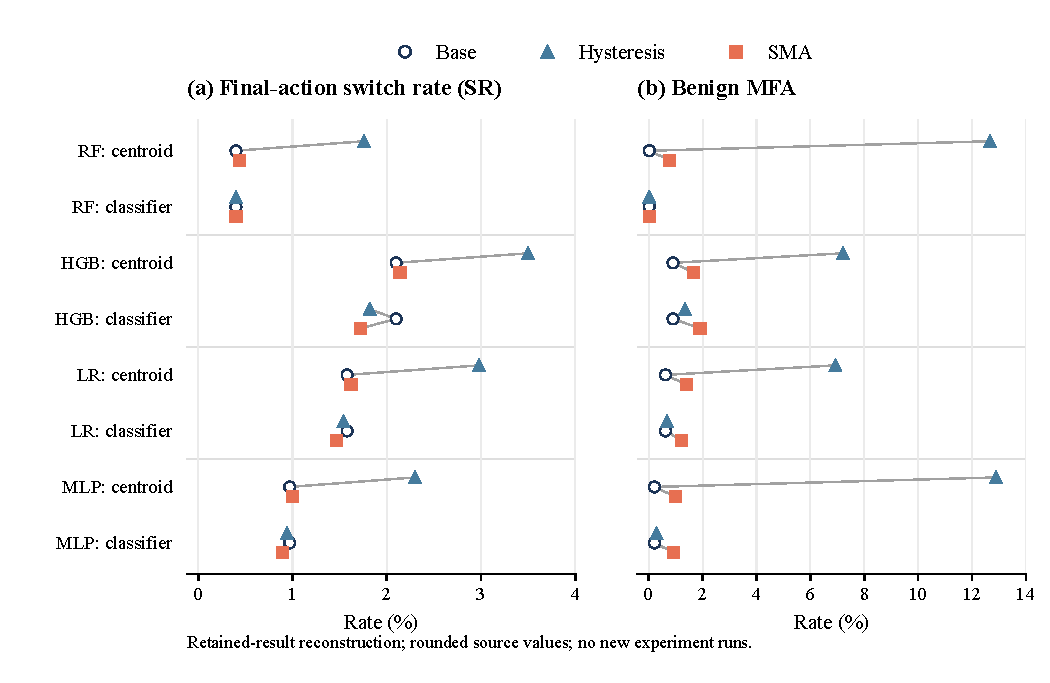
\includegraphics[width=\textwidth,height=4.7in,keepaspectratio]{figures/fig_supp_score_sources.pdf}
\caption{Evaluator and score-source sensitivity from the eight retained reconstruction rows. The two panels compare Base, Hysteresis and SMA final-action switch rates and benign-MFA rates for RF/HGB/LR/MLP under centroid and classifier scores. Horizontal positions reproduce the reported rounded percentages; vertical offsets separate overlapping symbols.}
\label{fig:supp_score_sources}
\end{figure}

Table~\ref{tab:supp_retained_evaluators} transcribes rounded
earlier Archive S9 results, separately from the purged
HGB candidate-bank replay in S3. For
centroid trust, hysteresis raises test final-action SR for
all four evaluators (HGB 2.10\% to 3.50\%); HGB benign
MFA becomes 7.21\%. Classifier-derived HGB trust instead
gives 2.10\% to 1.82\%, while equally budgeted SMA reaches
1.72\%. Software interface compatibility therefore does
not establish evaluator-independent performance gain.
Archive S9 retains full class-conditional rates, validation
burdens and adverse transfer screens.

\subsection{Retained original-topic PPO evaluator}
The submitted PPO weights were not recovered. A separate
new three-action PPO evaluator, seed 20260924, used
50,000 balanced early-training flows and a 197-component
transformed input. Its categorical Deny/MFA/Allow action
probabilities are not calibrated attack probabilities.
In that action order the proxy rewards are
\((-2,-0.25,+1)\) for benign labels and
\((+1,-0.5,-5)\) for attack labels, charging MFA for
both. Separate actor and critic networks have hidden
widths 256 and 128; their learning rates are
\(2\times10^{-4}\) and \(5\times10^{-4}\);
\(\gamma=0.99\), GAE \(0.95\), clipping \(0.20\),
entropy coefficient \(0.05\) to \(0.005\), and
gradient clipping \(0.5\). Each of 50 updates samples
1,024 early-train requests as four artificial 256-step
episodes, with four optimization epochs and minibatches
of 128. The next sampled flow is independent of the
selected action. This offline label reward is not a
deployed authentication feedback loop or a monotonic
PPO-improvement guarantee.

The frozen checkpoint was evaluated on 253,953 later
validation and 762,000 test flows. All conservative
fusion diagnostics in Table~\ref{tab:supp_retained_ppo}
fail the validation 5\% benign-MFA screen. Fixed
40/60 hysteresis raises test SR from 1.601\% to
2.625\%. Zero direct attack-Allow coexists with
19.159\% hard benign-Deny. On this one-seed proxy
trace, the reconstructed PPO comparator shows no
stabilization advantage.
\begin{table}[!htbp]
\centering
\caption{Retained single-seed original-topic three-action PPO evaluator on 762,000 chronological UNSW flows (percent). All policies fail the validation 5\% benign-MFA screen; entries are diagnostics, not eligible operating points. No result is from the later sequential-factor PPO study.}
\label{tab:supp_retained_ppo}
\scriptsize
\setlength{\tabcolsep}{3pt}
\begin{tabular}{lrrrrrr}
\toprule
Method & Val. MFA$_b$ & Test SR & Test FAR$_d$ & Test FDR$_h$ & Test MFA$_b$ & Test strict Acc.\\
\midrule
PPO base & 6.353 & 1.601 & 0.000 & 19.159 & 3.915 & 81.424 \\
Fixed 40/60 & 7.189 & 2.625 & 0.000 & 19.159 & 4.814 & 80.700 \\
Single & 6.617 & 2.058 & 0.000 & 19.159 & 4.215 & 81.182 \\
SMA & 6.353 & 1.602 & 0.000 & 19.159 & 3.915 & 81.424 \\
EMA & 6.353 & 1.601 & 0.000 & 19.159 & 3.915 & 81.424 \\
GP-LCB Hyst & 6.353 & 1.601 & 0.000 & 19.159 & 3.915 & 81.424 \\
\bottomrule
\end{tabular}
\end{table}

The separate ten-seed balanced static PPO study has no
valid temporal SR. Its NF-ToN-IoT-v2 FAR, hard FDR,
benign MFA and strict accuracy (mean \(\pm\) sample SD,
percent) are \(4.68\pm0.56\), \(17.88\pm4.28\),
\(13.84\pm5.84\) and \(80.10\pm2.07\).
UNSW-NB15 gives \(0.03\pm0.06\), \(1.96\pm0.29\),
\(0.87\pm1.40\) and \(98.46\pm0.73\); an exact-feature-
vector-disjoint UNSW sensitivity gives \(0.04\pm0.03\),
\(2.22\pm0.94\), \(2.68\pm3.05\) and \(97.20\pm1.87\).
These samples and protocols are distinct from the
one-seed chronological PPO diagnostic.

\subsection{Retained static NF-ToN-IoT-v2 prior stress and recheck}
NF-ToN-IoT-v2~\cite{nf_v2} has flow labels but lacks a defensible
absolute access-request timeline. Ten fixed seeds fit
RF, HGB, LR and MLP on earlier balanced samples.
After validation thresholds were locked, each model
scored the same previously constructed 100,000-row holdout
(50,000 benign and 50,000 attacks), whose original
row IDs are disjoint from every earlier prepared seed
sample. The 95/5 and 99/1 exercises retain all
50,000 benign rows and draw 2,632 or 505 attacks
by seeded row-ID hashing. Calibrated probabilities
receive a Bayes-odds correction under the explicit
pure-prior-shift assumption. Separate validation
thresholds are locked for each target prior before
the holdout is opened. These are paired resamples of
one corpus, not three independent populations.

An independent audit reread all 40 saved prediction
CSVs; verified holdout, threshold-lock and prediction
hashes; recomputed all 120 seed/model/prior action-count
cells; and matched reported counts/rates to
\(10^{-12}\). Table~\ref{tab:supp_nf_static} adds attack
MFA to the archived Table S15. LR's low direct
attack-Allow comes with 91.751\% benign MFA
and over 71\% attack MFA. Some seeds exceed a
0.5\% direct-FAR target under prior stress.
The table reports static class-conditional outcomes;
temporal switching and gateway execution have their
own protocols below.
% Static flow-label proxy outcomes; no chronology, SR or temporal cost.
% Requires booktabs. Three horizontal rules, no vertical rules.
\begin{suppnonfloattable}
\centering
\caption{Previously constructed row-disjoint NF-ToN-IoT-v2 static holdout under class-prior stress. Ten fixed training seeds; means across seeds. Thresholds were frozen on validation before scoring the new holdout. The 95/5 and 99/1 rows retain 50,000 benign flows and resample attack flows under a pure-prior-shift assumption. FAR is direct attack Allow; hard FDR is benign Deny; MFA rates are class conditional; strict accuracy credits benign Allow and attack Deny only. These flow-label proxies do not measure authentication completion, switch rate, or temporal cost.}
\label{tab:supp_nf_static}
\scriptsize
\setlength{\tabcolsep}{3.5pt}
\begin{tabular}{llrrrrrr}
\toprule
Evaluator & Attack prior & Attack $n$ & FAR (\%) & Hard FDR (\%) & Benign MFA (\%) & Attack MFA (\%) & Strict Acc. (\%) \\
\midrule
RF & 50\% & 50,000 & 0.235 & 3.740 & 0.000 & 0.000 & 98.012 \\
RF & 5\% & 2,632 & 0.266 & 3.720 & 0.000 & 0.000 & 96.453 \\
RF & 1\% & 505 & 0.396 & 3.720 & 0.000 & 0.000 & 96.314 \\
HGB & 50\% & 50,000 & 0.258 & 4.402 & 0.003 & 0.000 & 97.668 \\
HGB & 5\% & 2,632 & 0.255 & 4.373 & 0.003 & 0.000 & 95.830 \\
HGB & 1\% & 505 & 0.337 & 4.372 & 0.003 & 0.000 & 95.665 \\
LR & 50\% & 50,000 & 0.238 & 4.987 & 91.751 & 71.667 & 15.679 \\
LR & 5\% & 2,632 & 0.281 & 4.987 & 91.751 & 71.809 & 4.495 \\
LR & 1\% & 505 & 0.297 & 4.987 & 91.751 & 71.069 & 3.516 \\
MLP & 50\% & 50,000 & 0.338 & 5.115 & 3.855 & 0.560 & 95.066 \\
MLP & 5\% & 2,632 & 0.300 & 5.115 & 3.855 & 0.593 & 91.434 \\
MLP & 1\% & 505 & 0.376 & 5.115 & 3.855 & 0.733 & 91.108 \\
\bottomrule
\end{tabular}
\end{suppnonfloattable}


\section{Finite controls, static outcomes, and all feedback rows}
\label{sec:supp_results}

\subsection{Candidate bank and static selection}
The frozen bank contains 50 candidates per family:
hysteresis, single-threshold gating, SMA, EMA, and a
consecutive base-Allow counter. All 250 literal parameter
records and coordinates are in
\texttt{experiments/protocol.lock.json}. For each of the
first four families, four declared anchors precede 46
two-dimensional Latin-hypercube points with seed
\(20261008+j\), \(j=0,1,2,3\). With \(a,b\in[0,1]\),
hysteresis sets
\[
 \theta_{\rm low}=\operatorname{round}(99.9a,6),\quad
 \theta_{\rm high}=\operatorname{round}
 (\theta_{\rm low}+0.1+(99.9-\theta_{\rm low})b,6).
\]
Single gating uses \(\operatorname{round}(100a,6)\);
SMA uses that threshold and
\(\min(64,1+\lfloor64b\rfloor)\) events;
EMA uses that threshold and
\(\operatorname{round}(\exp[\log(0.01)(1-b)],6)\).
The counter family contains every \(K=1,\ldots,50\)
once, with \(K=1,2,8,50\) first. This generator,
its anchors, rounded values and selected IDs are
included in the frozen source and table CSV.
All candidates preserve base Deny and MFA and may
only restrict base Allow to pending MFA. New source-IP
groups start Low; SMA uses available within-group
history and EMA starts from its first group score.

Static calibration exhaustively evaluates 50 candidates
per family on the purged 253,933-event validation
trace. Eligibility requires direct attack-Allow
\(\le0.5\%\), hard benign-Deny \(\le5\%\), and
benign MFA \(\le\rho\) for
\(\rho\in\{1,2,5\}\%\).
Among feasible candidates, minimum final-action SR
wins; ties use lower benign MFA, direct FAR and
fixed candidate ID. No feasible candidate means
no selection, not a relaxed screen. Static choice
is a finite-bank exhaustive search, not BO and
not a continuous threshold optimum.

The base test action mix is 149,212 Deny,
8,944 MFA and 603,844 Allow over 762,000 events.
It makes 16,163 switches across 761,960 within-proxy
edges. Its 0.8812\% direct attack-Allow exceeds
the 0.5\% screen. At the 1\% benign-MFA cap,
none of the five families has a feasible validation
candidate. Table~\ref{tab:supp_static_all} reports
all 15 family/cap cells, including null selections
and simple controls with lower test SR than hysteresis.
\begin{table}[!htbp]
\centering
\caption{All 15 static validation family/cap outcomes on the purged HGB UNSW trace. Cap and rates are percent; cost uses declared proxy units. All 2\% and 5\% rows use the validation-selected candidate unchanged on test. At 1\% none is feasible on validation, so test endpoints are intentionally absent. Hard FDR is 0.853\% for each selected test row. Full numerators, denominators and candidate parameters are in the paired artifact CSV.}
\label{tab:supp_static_all}
\scriptsize
\setlength{\tabcolsep}{3pt}
\begin{tabular}{llrlrrrrrrl}
\toprule
Cap & Family & Val. feasible & Selected ID & SR & FAR$_d$ & MFA$_b$ & MFA$_a$ & Strict Acc. & Cost & Test caps\\
\midrule
1 & Hyst & 0 & -- & -- & -- & -- & -- & -- & -- & NA \\
1 & Single & 0 & -- & -- & -- & -- & -- & -- & -- & NA \\
1 & SMA & 0 & -- & -- & -- & -- & -- & -- & -- & NA \\
1 & EMA & 0 & -- & -- & -- & -- & -- & -- & -- & NA \\
1 & Counter & 0 & -- & -- & -- & -- & -- & -- & -- & NA \\
2 & Hyst & 21 & hysteresis\_27 & 1.826 & 0.036 & 1.417 & 3.042 & 97.572 & 0.01282 & Yes \\
2 & Single & 9 & single\_28 & 1.878 & 0.021 & 1.436 & 3.058 & 97.557 & 0.01259 & Yes \\
2 & SMA & 30 & sma\_10 & 1.749 & 0.053 & 1.799 & 3.025 & 97.265 & 0.01387 & Yes \\
2 & EMA & 27 & ema\_42 & 1.759 & 0.071 & 1.769 & 3.008 & 97.289 & 0.01415 & Yes \\
2 & Counter & 3 & counter\_05\_k4 & 1.809 & 0.190 & 1.768 & 2.889 & 97.290 & 0.01644 & Yes \\
5 & Hyst & 22 & hysteresis\_27 & 1.826 & 0.036 & 1.417 & 3.042 & 97.572 & 0.01282 & Yes \\
5 & Single & 10 & single\_21 & 1.779 & 0.000 & 2.192 & 3.078 & 96.948 & 0.01367 & Yes \\
5 & SMA & 38 & sma\_20 & 1.730 & 0.000 & 2.103 & 3.078 & 97.020 & 0.01346 & Yes \\
5 & EMA & 33 & ema\_06 & 1.729 & 0.000 & 2.120 & 3.078 & 97.007 & 0.01350 & Yes \\
5 & Counter & 49 & counter\_47\_k47 & 1.733 & 0.032 & 2.251 & 3.046 & 96.901 & 0.01438 & Yes \\
\bottomrule
\end{tabular}
\end{table}


\subsection{Causal label feedback and actual query budget}
The separate adaptive GP-LCB replay uses the same
250 continuously shadowed candidate policies, a
trailing 16,384-event window and scheduled updates
every 4,096 global events, beginning at event 4,096.
Each update needs 200 arrived benign labels,
20 arrived attack labels and 10\% arrived-label
coverage. At zero-based event index \(i\), scheduled
feedback for earlier event \(j=i-1-D\) can arrive;
a boundary update at \(i=4096,8192,\ldots\) uses
only events with index less than \(i\). The selected
version then governs action \(i\). Its own label is
scheduled only after that action commits, so even
\(D=0\) cannot change action \(i\). The first three conditions
in Table~\ref{tab:supp_feedback} were in the primary
lock. The isolated 25\%-clean and full-noisy
conditions were frozen in a post-primary addendum,
after primary results were inspected.

Within a supported family/window, four fixed anchors
and six GP-LCB acquisitions reveal ten candidate
losses. The separate per-family Gaussian process uses
fixed Mat\'ern-\(5/2\) length scale 0.2, constant
factor one, white-noise term \(10^{-5}\), ridge
\(10^{-6}\), normalized targets and acquisition
\(\mu-2\sigma\); it is rebuilt in each window.
Here \(\mu\) is the GP posterior predictive mean of the penalized loss
and \(\sigma\) its predictive standard deviation.
The queried score, with rates as fractions, is
\[
 L_\rho={\rm SR}_{a}
 +200[{\rm FAR}_{d}-0.005]_+
 +50[{\rm FDR}_{h}-0.05]_+
 +5[{\rm MFA}_{b}-\rho]_+ .
\]
At a scheduled boundary, a candidate commits for
event \(i\) only if its arrived-label rates pass all
screens; otherwise the incumbent remains, or the
base before the first commit. Each candidate's
scoped shadow state advances continuously and
version-edge action changes count toward SR.
All five conditions have 186 nominally supported
updates. Coverage, label flipping, exact scheduled
label counts and update support appear in
Table~\ref{tab:supp_feedback}.
\begin{table}[!htbp]
\centering
\caption{Locked and additive label-arrival conditions. Delay is in global events; the current label can arrive no earlier than the next event even at D0. The last two conditions were added after primary results were inspected. Support counts do not imply feasible candidate selection.}
\label{tab:supp_feedback}
\scriptsize
\setlength{\tabcolsep}{3pt}
\begin{tabular}{lrrrrrrr}
\toprule
Condition & Delay & Coverage & Flip & Updates & Supported & Scheduled labels & Flipped labels\\
\midrule
Full clean, D0 & 0 & 100 & 0 & 186 & 186 & 762,000 & 0 \\
Full clean, D256 & 256 & 100 & 0 & 186 & 186 & 762,000 & 0 \\
25\% clean, D256 & 256 & 25 & 0 & 186 & 186 & 190,274 & 0 \\
Full 10\% flip, D256 & 256 & 100 & 10 & 186 & 186 & 762,000 & 75,814 \\
25\% 10\% flip, D256 & 256 & 25 & 10 & 186 & 186 & 191,148 & 19,105 \\
\bottomrule
\end{tabular}
\end{table}


The ten-loss limit is an \emph{information disclosure}
budget, not ten objective computations. All
250 candidate action traces and all candidate
window metrics were computed as shadows before
selected losses reached the GP. Three primary
conditions disclose 83,700 losses but compute
139,500 full-bank candidate-window vectors;
two additive conditions add 55,800 and 93,000.
Across five conditions the totals are 139,500
loss disclosures and 232,500 metric vectors.
The budget controls loss disclosure while
computational work uses full shadows. Feedback
is injected from existing flow labels.

\begin{figure}[!t]
\centering
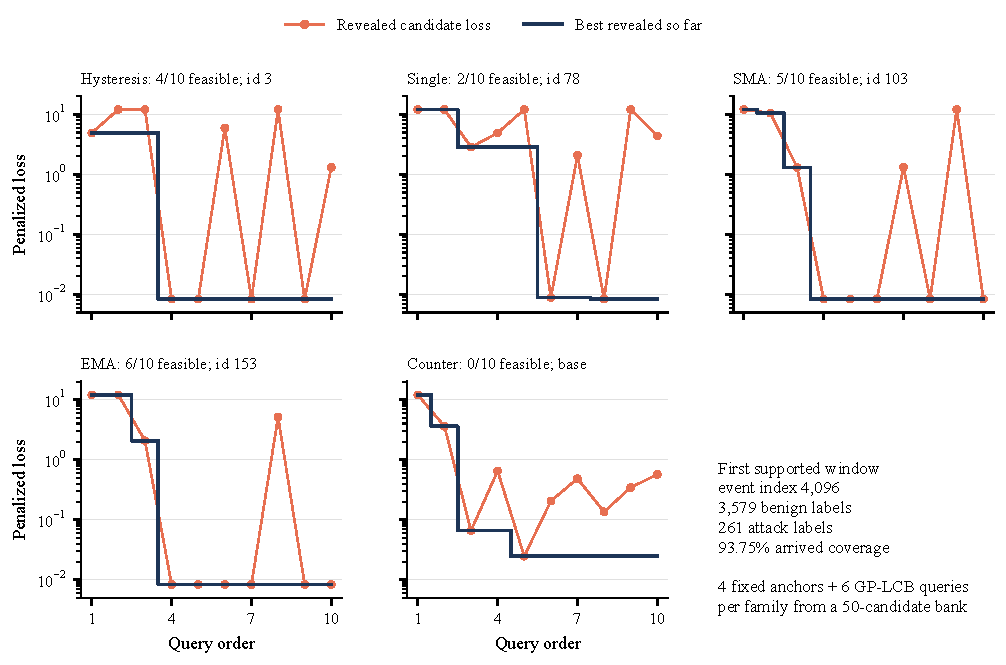
\includegraphics[width=\textwidth,height=5.0in,keepaspectratio]{figures/fig_supp_queries.pdf}
\caption{The ten saved GP-LCB loss queries at the first supported clean-D256 update, zero-based event index 4096, with a 2\% benign-MFA cap. Points are losses revealed to the surrogate; steps are the smallest revealed loss so far. Loss uses the declared penalized acquisition score. Titles give feasible queried counts and selected candidate IDs. All 50 shadow candidates were precomputed per family; this is a finite query-path diagnostic.}
\label{fig:supp_queries}
\end{figure}

\subsection{All 75 dynamic cells and negative controls}
Tables~\ref{tab:supp_dynamic_1}--\ref{tab:supp_dynamic_5}
report the full \(5\) feedback conditions
\(\times\,3\) benign-MFA caps \(\times\,5\) families.
No 1\%-cap
dynamic row meets the test screens. Under both
10\%-flipped feedback conditions, all 186
windows pass nominal support but no queried
candidate passes the arrived-label screens.
All families and caps remain on the unmodified
base with zero version commits; its direct FAR
remains 0.8812\% and fails the 0.5\% cap.
With 25\% clean feedback instead, commits occur.
These fixed conditions isolate the observed
effect of label corruption from missing coverage.
\begin{table}[!htbp]
\centering
\caption{All 25 causal feedback rows at the 1\% benign-MFA cap. Rates are percent; cost is a declared proxy. FDR is 0.853\% for every row because conservative fusion preserves base Deny. All 186 update windows per condition pass the nominal support gate. Zero-commit noisy rows remain on the base, which fails the direct-FAR cap. The two post-primary conditions are descriptive addenda.}
\label{tab:supp_dynamic_1}
\scriptsize
\setlength{\tabcolsep}{3pt}
\begin{tabular}{llrrrrrrrl}
\toprule
Condition & Family & SR & FAR$_d$ & MFA$_b$ & MFA$_a$ & Strict Acc. & Cost & Commits & Caps\\
\midrule
Full clean, D0 & Hyst & 1.870 & 0.135 & 1.478 & 2.944 & 97.523 & 0.01484 & 37 & No \\
Full clean, D0 & Single & 1.966 & 0.255 & 1.258 & 2.823 & 97.701 & 0.01673 & 33 & No \\
Full clean, D0 & SMA & 1.884 & 0.320 & 1.412 & 2.758 & 97.576 & 0.01824 & 54 & No \\
Full clean, D0 & EMA & 1.917 & 0.364 & 1.418 & 2.714 & 97.572 & 0.01910 & 52 & No \\
Full clean, D0 & Counter & 1.943 & 0.444 & 1.381 & 2.635 & 97.602 & 0.02055 & 35 & No \\
Full clean, D256 & Hyst & 1.870 & 0.135 & 1.478 & 2.944 & 97.523 & 0.01484 & 37 & No \\
Full clean, D256 & Single & 1.966 & 0.243 & 1.264 & 2.835 & 97.696 & 0.01651 & 31 & No \\
Full clean, D256 & SMA & 1.882 & 0.317 & 1.416 & 2.761 & 97.573 & 0.01818 & 56 & No \\
Full clean, D256 & EMA & 1.901 & 0.329 & 1.447 & 2.749 & 97.548 & 0.01849 & 53 & No \\
Full clean, D256 & Counter & 1.932 & 0.427 & 1.400 & 2.651 & 97.586 & 0.02028 & 35 & No \\
25\% clean, D256 & Hyst & 1.854 & 0.116 & 1.446 & 2.963 & 97.549 & 0.01441 & 44 & No \\
25\% clean, D256 & Single & 1.972 & 0.251 & 1.251 & 2.827 & 97.706 & 0.01664 & 24 & No \\
25\% clean, D256 & SMA & 1.880 & 0.347 & 1.426 & 2.732 & 97.565 & 0.01877 & 51 & No \\
25\% clean, D256 & EMA & 1.863 & 0.296 & 1.628 & 2.782 & 97.402 & 0.01821 & 53 & No \\
25\% clean, D256 & Counter & 1.916 & 0.407 & 1.526 & 2.672 & 97.484 & 0.02013 & 39 & No \\
Full 10\% flip, D256 & Hyst & 2.121 & 0.881 & 0.926 & 2.197 & 97.968 & 0.02804 & 0 & No \\
Full 10\% flip, D256 & Single & 2.121 & 0.881 & 0.926 & 2.197 & 97.968 & 0.02804 & 0 & No \\
Full 10\% flip, D256 & SMA & 2.121 & 0.881 & 0.926 & 2.197 & 97.968 & 0.02804 & 0 & No \\
Full 10\% flip, D256 & EMA & 2.121 & 0.881 & 0.926 & 2.197 & 97.968 & 0.02804 & 0 & No \\
Full 10\% flip, D256 & Counter & 2.121 & 0.881 & 0.926 & 2.197 & 97.968 & 0.02804 & 0 & No \\
25\% 10\% flip, D256 & Hyst & 2.121 & 0.881 & 0.926 & 2.197 & 97.968 & 0.02804 & 0 & No \\
25\% 10\% flip, D256 & Single & 2.121 & 0.881 & 0.926 & 2.197 & 97.968 & 0.02804 & 0 & No \\
25\% 10\% flip, D256 & SMA & 2.121 & 0.881 & 0.926 & 2.197 & 97.968 & 0.02804 & 0 & No \\
25\% 10\% flip, D256 & EMA & 2.121 & 0.881 & 0.926 & 2.197 & 97.968 & 0.02804 & 0 & No \\
25\% 10\% flip, D256 & Counter & 2.121 & 0.881 & 0.926 & 2.197 & 97.968 & 0.02804 & 0 & No \\
\bottomrule
\end{tabular}
\end{table}

\begin{table}[!htbp]
\centering
\caption{All 25 causal feedback rows at the 2\% benign-MFA cap. Rates are percent; cost is a declared proxy. FDR is 0.853\% for every row because conservative fusion preserves base Deny. All 186 update windows per condition pass the nominal support gate. Zero-commit noisy rows remain on the base, which fails the direct-FAR cap. The two post-primary conditions are descriptive addenda.}
\label{tab:supp_dynamic_2}
\scriptsize
\setlength{\tabcolsep}{3pt}
\begin{tabular}{llrrrrrrrl}
\toprule
Condition & Family & SR & FAR$_d$ & MFA$_b$ & MFA$_a$ & Strict Acc. & Cost & Commits & Caps\\
\midrule
Full clean, D0 & Hyst & 1.850 & 0.078 & 1.443 & 3.000 & 97.551 & 0.01368 & 68 & Yes \\
Full clean, D0 & Single & 1.945 & 0.192 & 1.291 & 2.887 & 97.674 & 0.01559 & 44 & Yes \\
Full clean, D0 & SMA & 1.820 & 0.256 & 1.534 & 2.823 & 97.478 & 0.01723 & 78 & Yes \\
Full clean, D0 & EMA & 1.810 & 0.106 & 1.689 & 2.973 & 97.353 & 0.01468 & 61 & Yes \\
Full clean, D0 & Counter & 1.835 & 0.230 & 1.681 & 2.848 & 97.360 & 0.01705 & 62 & Yes \\
Full clean, D256 & Hyst & 1.852 & 0.079 & 1.439 & 2.999 & 97.555 & 0.01370 & 67 & Yes \\
Full clean, D256 & Single & 1.946 & 0.193 & 1.291 & 2.886 & 97.674 & 0.01560 & 46 & Yes \\
Full clean, D256 & SMA & 1.820 & 0.258 & 1.534 & 2.821 & 97.478 & 0.01727 & 78 & Yes \\
Full clean, D256 & EMA & 1.812 & 0.104 & 1.702 & 2.975 & 97.343 & 0.01467 & 63 & Yes \\
Full clean, D256 & Counter & 1.824 & 0.217 & 1.703 & 2.862 & 97.342 & 0.01683 & 62 & Yes \\
25\% clean, D256 & Hyst & 1.861 & 0.087 & 1.499 & 2.992 & 97.506 & 0.01397 & 61 & Yes \\
25\% clean, D256 & Single & 1.967 & 0.221 & 1.273 & 2.857 & 97.688 & 0.01612 & 27 & Yes \\
25\% clean, D256 & SMA & 1.842 & 0.248 & 1.610 & 2.831 & 97.417 & 0.01724 & 71 & Yes \\
25\% clean, D256 & EMA & 1.864 & 0.224 & 1.556 & 2.854 & 97.460 & 0.01669 & 61 & Yes \\
25\% clean, D256 & Counter & 1.851 & 0.278 & 1.693 & 2.800 & 97.350 & 0.01799 & 61 & Yes \\
Full 10\% flip, D256 & Hyst & 2.121 & 0.881 & 0.926 & 2.197 & 97.968 & 0.02804 & 0 & No \\
Full 10\% flip, D256 & Single & 2.121 & 0.881 & 0.926 & 2.197 & 97.968 & 0.02804 & 0 & No \\
Full 10\% flip, D256 & SMA & 2.121 & 0.881 & 0.926 & 2.197 & 97.968 & 0.02804 & 0 & No \\
Full 10\% flip, D256 & EMA & 2.121 & 0.881 & 0.926 & 2.197 & 97.968 & 0.02804 & 0 & No \\
Full 10\% flip, D256 & Counter & 2.121 & 0.881 & 0.926 & 2.197 & 97.968 & 0.02804 & 0 & No \\
25\% 10\% flip, D256 & Hyst & 2.121 & 0.881 & 0.926 & 2.197 & 97.968 & 0.02804 & 0 & No \\
25\% 10\% flip, D256 & Single & 2.121 & 0.881 & 0.926 & 2.197 & 97.968 & 0.02804 & 0 & No \\
25\% 10\% flip, D256 & SMA & 2.121 & 0.881 & 0.926 & 2.197 & 97.968 & 0.02804 & 0 & No \\
25\% 10\% flip, D256 & EMA & 2.121 & 0.881 & 0.926 & 2.197 & 97.968 & 0.02804 & 0 & No \\
25\% 10\% flip, D256 & Counter & 2.121 & 0.881 & 0.926 & 2.197 & 97.968 & 0.02804 & 0 & No \\
\bottomrule
\end{tabular}
\end{table}

\begin{table}[!htbp]
\centering
\caption{All 25 causal feedback rows at the 5\% benign-MFA cap. Rates are percent; cost is a declared proxy. FDR is 0.853\% for every row because conservative fusion preserves base Deny. All 186 update windows per condition pass the nominal support gate. Zero-commit noisy rows remain on the base, which fails the direct-FAR cap. The two post-primary conditions are descriptive addenda.}
\label{tab:supp_dynamic_5}
\scriptsize
\setlength{\tabcolsep}{3pt}
\begin{tabular}{llrrrrrrrl}
\toprule
Condition & Family & SR & FAR$_d$ & MFA$_b$ & MFA$_a$ & Strict Acc. & Cost & Commits & Caps\\
\midrule
Full clean, D0 & Hyst & 1.838 & 0.044 & 1.626 & 3.035 & 97.404 & 0.01339 & 69 & Yes \\
Full clean, D0 & Single & 1.927 & 0.159 & 1.316 & 2.920 & 97.653 & 0.01500 & 43 & Yes \\
Full clean, D0 & SMA & 1.758 & 0.114 & 1.847 & 2.965 & 97.226 & 0.01513 & 60 & Yes \\
Full clean, D0 & EMA & 1.751 & 0.027 & 2.011 & 3.051 & 97.094 & 0.01380 & 44 & Yes \\
Full clean, D0 & Counter & 1.755 & 0.120 & 2.053 & 2.958 & 97.060 & 0.01567 & 64 & Yes \\
Full clean, D256 & Hyst & 1.836 & 0.041 & 1.644 & 3.037 & 97.390 & 0.01338 & 65 & Yes \\
Full clean, D256 & Single & 1.929 & 0.162 & 1.315 & 2.917 & 97.654 & 0.01505 & 43 & Yes \\
Full clean, D256 & SMA & 1.758 & 0.114 & 1.853 & 2.965 & 97.221 & 0.01514 & 61 & Yes \\
Full clean, D256 & EMA & 1.751 & 0.027 & 2.009 & 3.051 & 97.096 & 0.01380 & 44 & Yes \\
Full clean, D256 & Counter & 1.755 & 0.120 & 2.053 & 2.958 & 97.060 & 0.01567 & 65 & Yes \\
25\% clean, D256 & Hyst & 1.837 & 0.046 & 1.607 & 3.033 & 97.420 & 0.01339 & 65 & Yes \\
25\% clean, D256 & Single & 1.939 & 0.181 & 1.303 & 2.897 & 97.664 & 0.01540 & 32 & Yes \\
25\% clean, D256 & SMA & 1.757 & 0.110 & 1.870 & 2.968 & 97.207 & 0.01511 & 57 & Yes \\
25\% clean, D256 & EMA & 1.756 & 0.044 & 1.999 & 3.035 & 97.104 & 0.01410 & 45 & Yes \\
25\% clean, D256 & Counter & 1.759 & 0.125 & 2.045 & 2.953 & 97.066 & 0.01574 & 63 & Yes \\
Full 10\% flip, D256 & Hyst & 2.121 & 0.881 & 0.926 & 2.197 & 97.968 & 0.02804 & 0 & No \\
Full 10\% flip, D256 & Single & 2.121 & 0.881 & 0.926 & 2.197 & 97.968 & 0.02804 & 0 & No \\
Full 10\% flip, D256 & SMA & 2.121 & 0.881 & 0.926 & 2.197 & 97.968 & 0.02804 & 0 & No \\
Full 10\% flip, D256 & EMA & 2.121 & 0.881 & 0.926 & 2.197 & 97.968 & 0.02804 & 0 & No \\
Full 10\% flip, D256 & Counter & 2.121 & 0.881 & 0.926 & 2.197 & 97.968 & 0.02804 & 0 & No \\
25\% 10\% flip, D256 & Hyst & 2.121 & 0.881 & 0.926 & 2.197 & 97.968 & 0.02804 & 0 & No \\
25\% 10\% flip, D256 & Single & 2.121 & 0.881 & 0.926 & 2.197 & 97.968 & 0.02804 & 0 & No \\
25\% 10\% flip, D256 & SMA & 2.121 & 0.881 & 0.926 & 2.197 & 97.968 & 0.02804 & 0 & No \\
25\% 10\% flip, D256 & EMA & 2.121 & 0.881 & 0.926 & 2.197 & 97.968 & 0.02804 & 0 & No \\
25\% 10\% flip, D256 & Counter & 2.121 & 0.881 & 0.926 & 2.197 & 97.968 & 0.02804 & 0 & No \\
\bottomrule
\end{tabular}
\end{table}


The five fixed diagnostics in
Table~\ref{tab:supp_diagnostics} show why SR
or permissive accuracy alone is inadequate.
Always-MFA has zero SR and 100\% submitted-style
permissive accuracy, yet zero strict diagnostic
accuracy and a challenge for every flow.
Constant trust 50 under safe 40/60 fusion has
99.147\% benign MFA and 18.895\% strict
accuracy. That is a new ablation, not a
byte-identical reconstruction of the submitted
trust-masked PPO row. The original unsafe
bidirectional promotion, shown only as an
offline counterexample, raises direct
attack-Allow from base 0.881\% to 2.364\%;
it was excluded from eligible selection and
execution.
\begin{table}[!htbp]
\centering
\caption{Fixed ablations and negative controls on the same UNSW test trace. Permissive accuracy credits MFA for either class and is shown solely to expose the submitted definition's failure. Unsafe legacy fusion is offline only and was never eligible for selection or execution.}
\label{tab:supp_diagnostics}
\scriptsize
\setlength{\tabcolsep}{3pt}
\begin{tabular}{lrrrrrrr}
\toprule
Diagnostic & SR & FAR$_d$ & FDR$_h$ & MFA$_b$ & Strict Acc. & Permissive Acc. & Cost\\
\midrule
Base & 2.121 & 0.881 & 0.853 & 0.926 & 97.968 & 99.141 & 0.02804 \\
Always MFA & 0.000 & 0.000 & 0.000 & 100.000 & 0.000 & 100.000 & 0.25000 \\
Constant trust 50 & 1.729 & 0.000 & 0.853 & 99.147 & 18.895 & 99.313 & 0.20878 \\
Fixed Hyst 40/60 & 2.121 & 0.881 & 0.853 & 0.926 & 97.968 & 99.141 & 0.02804 \\
Unsafe legacy fusion & 1.829 & 2.364 & 0.794 & 0.264 & 98.520 & 98.900 & 0.05435 \\
\bottomrule
\end{tabular}
\end{table}


\subsection{Separately locked synthetic score-calibration shift}
\label{sec:supp_score_shift}
An additional protocol was locked on 9 October 2026
\emph{before} computing this diagnostic's outcomes
(SHA-256 prefix \texttt{dfb27373f83ee70b}).
It leaves the previously frozen 45 primary and
30 missing/noisy feedback rows byte-unchanged.
The 762,000 inspected UNSW test events are sorted
globally by observed start second and original row
ID and divided into four equal rank quarters of
190,500 events. Trust-score offsets
\((0,+12,-12,0)\) are applied and clipped to
\([0,100]\); the event labels, source-IP groups,
timestamps, row IDs, fitted evaluator and base
Deny/MFA/Allow actions are unchanged. Phase
boundaries occur at global ranks
190,500, 381,000 and 571,500. The transform
clips 151,682 high values in the \(+12\) quarter
and 35,273 low values in the \(-12\) quarter.
This is an \emph{abrupt constructed score-calibration
shift}, not measured traffic/concept drift or
recovery of the submitted drift generator.

The fixed comparison retains exactly the
unshifted-validation-selected five families at
2\% and 5\% benign-MFA caps. The adaptive
comparison reuses the same 250-candidate bank,
clean feedback with 256-global-event label delay,
the frozen 16,384/4,096 window and cadence,
support gate and ten-disclosed-loss GP-LCB rule.
There is no test-stage threshold selection.
All 20 full-trace method/cap/mode combinations
appear in Table~\ref{tab:supp_shift_all20}.
The 80 quarter-level rows appear without
omission in
Tables~\ref{tab:supp_shift_phase_2_fixed}--
\ref{tab:supp_shift_phase_5_adaptive}.
An eligible within-source-IP edge belongs to
the quarter of its \emph{later} event. The
audit counts 96 cross-quarter within-proxy
edges, rather than silently dropping them;
the machine CSV also records action switches
on those edges and on version boundaries.

At the 2\% cap, fixed hysteresis has
whole-trace SR 1.8401\%, direct FAR 0.1373\%,
and benign MFA 1.5467\%. Adaptive hysteresis
has 1.8799\%, 0.1542\% and 1.9042\%,
respectively: no improvement on these
aggregate coordinates. In the \(-12\) quarter,
their benign-MFA rates are 2.1607\% and
3.4472\%, so both violate that phase's
2\% burden screen despite passing the
whole-trace test cap. At the 5\% cap,
fixed SMA and EMA each exceed 26\% benign
MFA under this shift; adaptive versions
lower their aggregate burden to about
2.1--2.2\% but have higher SR.
The outcome is method- and endpoint-dependent.
The previously inspected source-IP-proxy test
makes this an exploratory sensitivity. An
independent audit checks
1,360 metrics and counts, including
480 boundary items, across the 20 method
and 80 phase rows. The score-shift GP
receives 18,600 queried losses while
46,500 full-bank candidate-window metric
vectors are computed; no runtime efficiency
claim follows.
\begin{table}[!htbp]
\centering
\caption{All 20 whole-trace policy rows of the separately locked synthetic score-offset sensitivity. Fixed candidates retain unshifted-validation selections; adaptive policies use clean D256 feedback, the unchanged 250-policy shadow bank and no test-stage selection. Rates are percent; cost is a declared proxy. Phase failures count failing quarter-level safety/MFA screens. FDR is 0.853\% for every row.}
\label{tab:supp_shift_all20}
\scriptsize
\setlength{\tabcolsep}{2.6pt}
\begin{tabular}{lllrrrrrrrl}
\toprule
Mode & Cap & Family & SR & FAR$_d$ & MFA$_b$ & MFA$_a$ & Cost & Commits & Phase failures & Full caps\\
\midrule
Fixed & 2 & Hyst & 1.840 & 0.137 & 1.547 & 2.941 & 0.01501 & 0 & 1 & Yes \\
Adaptive & 2 & Hyst & 1.880 & 0.154 & 1.904 & 2.924 & 0.01607 & 59 & 1 & Yes \\
Fixed & 2 & Single & 1.886 & 0.158 & 25.687 & 2.921 & 0.06400 & 0 & 2 & No \\
Adaptive & 2 & Single & 2.033 & 0.563 & 1.112 & 2.515 & 0.02233 & 27 & 2 & No \\
Fixed & 2 & SMA & 1.752 & 0.072 & 1.858 & 3.006 & 0.01435 & 0 & 1 & Yes \\
Adaptive & 2 & SMA & 1.829 & 0.222 & 1.925 & 2.856 & 0.01738 & 79 & 1 & Yes \\
Fixed & 2 & EMA & 1.761 & 0.088 & 1.823 & 2.991 & 0.01458 & 0 & 1 & Yes \\
Adaptive & 2 & EMA & 1.823 & 0.154 & 1.799 & 2.924 & 0.01583 & 66 & 1 & Yes \\
Fixed & 2 & Counter & 1.809 & 0.190 & 1.768 & 2.889 & 0.01644 & 0 & 0 & Yes \\
Adaptive & 2 & Counter & 1.824 & 0.217 & 1.703 & 2.862 & 0.01683 & 62 & 0 & Yes \\
Fixed & 5 & Hyst & 1.840 & 0.137 & 1.547 & 2.941 & 0.01501 & 0 & 0 & Yes \\
Adaptive & 5 & Hyst & 1.857 & 0.122 & 2.134 & 2.957 & 0.01591 & 53 & 0 & Yes \\
Fixed & 5 & Single & 1.826 & 0.075 & 26.116 & 3.003 & 0.06327 & 0 & 1 & No \\
Adaptive & 5 & Single & 2.017 & 0.454 & 1.154 & 2.625 & 0.02032 & 26 & 1 & Yes \\
Fixed & 5 & SMA & 1.735 & 0.000 & 26.352 & 3.078 & 0.06227 & 0 & 1 & No \\
Adaptive & 5 & SMA & 1.768 & 0.069 & 2.196 & 3.010 & 0.01498 & 68 & 0 & Yes \\
Fixed & 5 & EMA & 1.734 & 0.000 & 26.469 & 3.078 & 0.06251 & 0 & 1 & No \\
Adaptive & 5 & EMA & 1.769 & 0.051 & 2.104 & 3.027 & 0.01446 & 52 & 0 & Yes \\
Fixed & 5 & Counter & 1.733 & 0.032 & 2.251 & 3.046 & 0.01438 & 0 & 0 & Yes \\
Adaptive & 5 & Counter & 1.755 & 0.120 & 2.053 & 2.958 & 0.01567 & 65 & 0 & Yes \\
\bottomrule
\end{tabular}
\end{table}

\begin{figure}[!t]
\centering
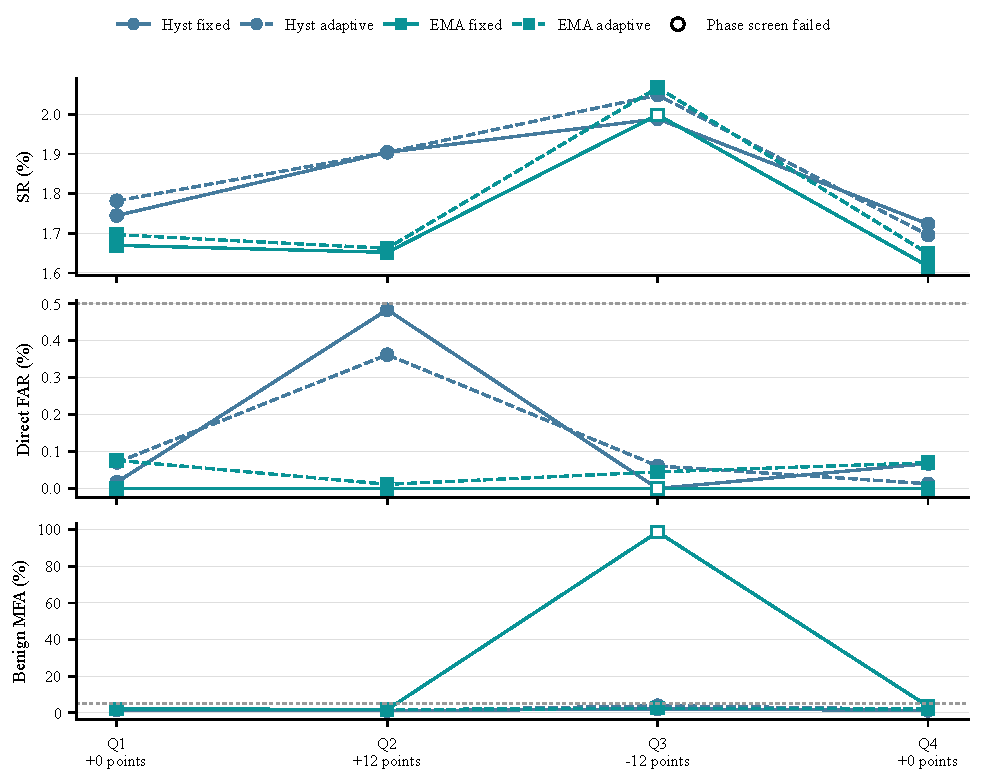
\includegraphics[width=\textwidth,height=5.6in,keepaspectratio]{figures/fig_supp_score_shift5.pdf}
\caption{Fixed and adaptive hysteresis/EMA under the 5\% benign-MFA cap in the same four-quarter calibration stress. Offsets are $0,+12,-12,0$ on unchanged flows and base actions. Open markers identify phase-screen failures. The negative-offset quarter exposes the high fixed-EMA verification burden and the different adaptive operating point.}
\label{fig:supp_shift5}
\end{figure}

\begin{table}[!htbp]
\centering
\caption{All 20 quarter-level rows for the 2\% cap, fixed policy under synthetic score offsets 0,+12,-12,0. Each phase contains 190,500 events. Adjacent edges are assigned to the later event's phase, including cross-phase edges; full boundary counts and action changes are in the saved phase CSV. Rates are percent and cost is a proxy.}
\label{tab:supp_shift_phase_2_fixed}
\scriptsize
\setlength{\tabcolsep}{2.6pt}
\begin{tabular}{rrlrrrrrrl}
\toprule
Phase & Offset & Family & SR & FAR$_d$ & MFA$_b$ & MFA$_a$ & Strict Acc. & Cost & Caps\\
\midrule
1 & +0 & Hyst & 1.745 & 0.017 & 1.541 & 3.445 & 97.477 & 0.01217 & Yes \\
1 & +0 & Single & 1.776 & 0.014 & 1.565 & 3.448 & 97.458 & 0.01218 & Yes \\
1 & +0 & SMA & 1.683 & 0.068 & 1.913 & 3.394 & 97.174 & 0.01382 & Yes \\
1 & +0 & EMA & 1.693 & 0.076 & 1.887 & 3.386 & 97.195 & 0.01392 & Yes \\
1 & +0 & Counter & 1.747 & 0.206 & 1.892 & 3.256 & 97.192 & 0.01632 & Yes \\
2 & +12 & Hyst & 1.904 & 0.484 & 1.163 & 2.744 & 97.613 & 0.02198 & Yes \\
2 & +12 & Single & 1.944 & 0.611 & 1.212 & 2.617 & 97.573 & 0.02440 & No \\
2 & +12 & SMA & 1.678 & 0.144 & 1.726 & 3.083 & 97.154 & 0.01687 & Yes \\
2 & +12 & EMA & 1.689 & 0.198 & 1.701 & 3.030 & 97.175 & 0.01780 & Yes \\
2 & +12 & Counter & 1.707 & 0.229 & 1.652 & 2.999 & 97.215 & 0.01827 & Yes \\
3 & -12 & Hyst & 1.988 & 0.000 & 2.161 & 2.828 & 96.942 & 0.01438 & No \\
3 & -12 & Single & 2.002 & 0.000 & 99.045 & 2.828 & 19.266 & 0.20858 & No \\
3 & -12 & SMA & 1.990 & 0.000 & 2.155 & 2.828 & 96.946 & 0.01437 & No \\
3 & -12 & EMA & 1.993 & 0.000 & 2.126 & 2.828 & 96.970 & 0.01431 & No \\
3 & -12 & Counter & 2.055 & 0.217 & 1.868 & 2.611 & 97.176 & 0.01802 & Yes \\
4 & +0 & Hyst & 1.723 & 0.068 & 1.324 & 2.776 & 97.841 & 0.01151 & Yes \\
4 & +0 & Single & 1.822 & 0.033 & 1.328 & 2.811 & 97.838 & 0.01085 & Yes \\
4 & +0 & SMA & 1.656 & 0.080 & 1.637 & 2.763 & 97.594 & 0.01235 & Yes \\
4 & +0 & EMA & 1.670 & 0.083 & 1.575 & 2.761 & 97.643 & 0.01229 & Yes \\
4 & +0 & Counter & 1.728 & 0.115 & 1.658 & 2.728 & 97.577 & 0.01314 & Yes \\
\bottomrule
\end{tabular}
\end{table}

\begin{table}[!htbp]
\centering
\caption{All 20 quarter-level rows for the 2\% cap, adaptive policy under synthetic score offsets 0,+12,-12,0. Each phase contains 190,500 events. Adjacent edges are assigned to the later event's phase, including cross-phase edges; full boundary counts and action changes are in the saved phase CSV. Rates are percent and cost is a proxy.}
\label{tab:supp_shift_phase_2_adaptive}
\scriptsize
\setlength{\tabcolsep}{2.6pt}
\begin{tabular}{rrlrrrrrrl}
\toprule
Phase & Offset & Family & SR & FAR$_d$ & MFA$_b$ & MFA$_a$ & Strict Acc. & Cost & Caps\\
\midrule
1 & +0 & Hyst & 1.795 & 0.107 & 1.513 & 3.355 & 97.500 & 0.01378 & Yes \\
1 & +0 & Single & 1.842 & 0.152 & 1.461 & 3.310 & 97.542 & 0.01451 & Yes \\
1 & +0 & SMA & 1.771 & 0.288 & 1.690 & 3.174 & 97.356 & 0.01740 & Yes \\
1 & +0 & EMA & 1.737 & 0.166 & 1.930 & 3.296 & 97.161 & 0.01567 & Yes \\
1 & +0 & Counter & 1.757 & 0.262 & 1.890 & 3.200 & 97.193 & 0.01734 & Yes \\
2 & +12 & Hyst & 1.904 & 0.362 & 1.256 & 2.866 & 97.538 & 0.01997 & Yes \\
2 & +12 & Single & 2.032 & 0.965 & 0.984 & 2.263 & 97.759 & 0.03038 & No \\
2 & +12 & SMA & 1.721 & 0.099 & 1.615 & 3.129 & 97.245 & 0.01585 & Yes \\
2 & +12 & EMA & 1.707 & 0.082 & 1.620 & 3.146 & 97.240 & 0.01554 & Yes \\
2 & +12 & Counter & 1.714 & 0.286 & 1.609 & 2.942 & 97.249 & 0.01921 & Yes \\
3 & -12 & Hyst & 2.091 & 0.103 & 3.447 & 2.724 & 95.910 & 0.01901 & No \\
3 & -12 & Single & 2.333 & 0.752 & 0.930 & 2.076 & 97.929 & 0.02662 & No \\
3 & -12 & SMA & 2.088 & 0.238 & 2.995 & 2.589 & 96.272 & 0.02071 & No \\
3 & -12 & EMA & 2.111 & 0.196 & 2.177 & 2.632 & 96.929 & 0.01826 & No \\
3 & -12 & Counter & 2.098 & 0.222 & 1.698 & 2.605 & 97.312 & 0.01781 & Yes \\
4 & +0 & Hyst & 1.730 & 0.060 & 1.410 & 2.783 & 97.773 & 0.01153 & Yes \\
4 & +0 & Single & 1.924 & 0.395 & 1.071 & 2.448 & 98.041 & 0.01782 & Yes \\
4 & +0 & SMA & 1.734 & 0.258 & 1.401 & 2.586 & 97.780 & 0.01556 & Yes \\
4 & +0 & EMA & 1.735 & 0.168 & 1.466 & 2.676 & 97.729 & 0.01385 & Yes \\
4 & +0 & Counter & 1.727 & 0.110 & 1.613 & 2.733 & 97.613 & 0.01295 & Yes \\
\bottomrule
\end{tabular}
\end{table}

\begin{table}[!htbp]
\centering
\caption{All 20 quarter-level rows for the 5\% cap, fixed policy under synthetic score offsets 0,+12,-12,0. Each phase contains 190,500 events. Adjacent edges are assigned to the later event's phase, including cross-phase edges; full boundary counts and action changes are in the saved phase CSV. Rates are percent and cost is a proxy.}
\label{tab:supp_shift_phase_5_fixed}
\scriptsize
\setlength{\tabcolsep}{2.6pt}
\begin{tabular}{rrlrrrrrrl}
\toprule
Phase & Offset & Family & SR & FAR$_d$ & MFA$_b$ & MFA$_a$ & Strict Acc. & Cost & Caps\\
\midrule
1 & +0 & Hyst & 1.745 & 0.017 & 1.541 & 3.445 & 97.477 & 0.01217 & Yes \\
1 & +0 & Single & 1.724 & 0.000 & 2.263 & 3.462 & 96.889 & 0.01332 & Yes \\
1 & +0 & SMA & 1.670 & 0.000 & 2.148 & 3.462 & 96.983 & 0.01306 & Yes \\
1 & +0 & EMA & 1.670 & 0.000 & 2.206 & 3.462 & 96.935 & 0.01318 & Yes \\
1 & +0 & Counter & 1.680 & 0.000 & 2.713 & 3.462 & 96.523 & 0.01422 & Yes \\
2 & +12 & Hyst & 1.904 & 0.484 & 1.163 & 2.744 & 97.613 & 0.02198 & Yes \\
2 & +12 & Single & 1.912 & 0.317 & 1.274 & 2.911 & 97.522 & 0.01919 & Yes \\
2 & +12 & SMA & 1.652 & 0.000 & 1.837 & 3.228 & 97.064 & 0.01447 & Yes \\
2 & +12 & EMA & 1.652 & 0.000 & 1.814 & 3.228 & 97.083 & 0.01443 & Yes \\
2 & +12 & Counter & 1.653 & 0.048 & 1.876 & 3.180 & 97.032 & 0.01542 & Yes \\
3 & -12 & Hyst & 1.988 & 0.000 & 2.161 & 2.828 & 96.942 & 0.01438 & Yes \\
3 & -12 & Single & 2.002 & 0.000 & 99.045 & 2.828 & 19.266 & 0.20858 & No \\
3 & -12 & SMA & 2.002 & 0.000 & 98.995 & 2.828 & 19.306 & 0.20848 & No \\
3 & -12 & EMA & 1.998 & 0.000 & 98.717 & 2.828 & 19.529 & 0.20792 & No \\
3 & -12 & Counter & 1.989 & 0.077 & 2.167 & 2.751 & 96.937 & 0.01588 & Yes \\
4 & +0 & Hyst & 1.723 & 0.068 & 1.324 & 2.776 & 97.841 & 0.01151 & Yes \\
4 & +0 & Single & 1.665 & 0.000 & 2.290 & 2.843 & 97.078 & 0.01201 & Yes \\
4 & +0 & SMA & 1.617 & 0.000 & 2.841 & 2.843 & 96.643 & 0.01307 & Yes \\
4 & +0 & EMA & 1.617 & 0.000 & 3.565 & 2.843 & 96.071 & 0.01450 & Yes \\
4 & +0 & Counter & 1.609 & 0.005 & 2.247 & 2.838 & 97.112 & 0.01200 & Yes \\
\bottomrule
\end{tabular}
\end{table}

\begin{table}[!htbp]
\centering
\caption{All 20 quarter-level rows for the 5\% cap, adaptive policy under synthetic score offsets 0,+12,-12,0. Each phase contains 190,500 events. Adjacent edges are assigned to the later event's phase, including cross-phase edges; full boundary counts and action changes are in the saved phase CSV. Rates are percent and cost is a proxy.}
\label{tab:supp_shift_phase_5_adaptive}
\scriptsize
\setlength{\tabcolsep}{2.6pt}
\begin{tabular}{rrlrrrrrrl}
\toprule
Phase & Offset & Family & SR & FAR$_d$ & MFA$_b$ & MFA$_a$ & Strict Acc. & Cost & Caps\\
\midrule
1 & +0 & Hyst & 1.782 & 0.071 & 1.563 & 3.392 & 97.459 & 0.01321 & Yes \\
1 & +0 & Single & 1.837 & 0.150 & 1.477 & 3.313 & 97.529 & 0.01449 & Yes \\
1 & +0 & SMA & 1.704 & 0.079 & 1.904 & 3.383 & 97.182 & 0.01402 & Yes \\
1 & +0 & EMA & 1.696 & 0.076 & 2.071 & 3.386 & 97.046 & 0.01430 & Yes \\
1 & +0 & Counter & 1.718 & 0.155 & 2.189 & 3.307 & 96.949 & 0.01599 & Yes \\
2 & +12 & Hyst & 1.904 & 0.362 & 1.256 & 2.866 & 97.538 & 0.01997 & Yes \\
2 & +12 & Single & 2.032 & 0.965 & 0.984 & 2.263 & 97.759 & 0.03038 & No \\
2 & +12 & SMA & 1.678 & 0.037 & 1.789 & 3.191 & 97.103 & 0.01505 & Yes \\
2 & +12 & EMA & 1.662 & 0.011 & 1.799 & 3.216 & 97.095 & 0.01461 & Yes \\
2 & +12 & Counter & 1.668 & 0.201 & 1.787 & 3.027 & 97.104 & 0.01801 & Yes \\
3 & -12 & Hyst & 2.048 & 0.061 & 3.889 & 2.767 & 95.556 & 0.01905 & Yes \\
3 & -12 & Single & 2.310 & 0.442 & 1.019 & 2.386 & 97.857 & 0.02080 & Yes \\
3 & -12 & SMA & 2.024 & 0.019 & 3.261 & 2.809 & 96.060 & 0.01696 & Yes \\
3 & -12 & EMA & 2.067 & 0.045 & 2.512 & 2.783 & 96.660 & 0.01599 & Yes \\
3 & -12 & Counter & 2.003 & 0.071 & 2.098 & 2.756 & 96.992 & 0.01564 & Yes \\
4 & +0 & Hyst & 1.696 & 0.013 & 1.846 & 2.831 & 97.429 & 0.01140 & Yes \\
4 & +0 & Single & 1.891 & 0.283 & 1.133 & 2.561 & 97.992 & 0.01562 & Yes \\
4 & +0 & SMA & 1.666 & 0.135 & 1.837 & 2.708 & 97.436 & 0.01388 & Yes \\
4 & +0 & EMA & 1.649 & 0.070 & 2.039 & 2.773 & 97.276 & 0.01294 & Yes \\
4 & +0 & Counter & 1.631 & 0.065 & 2.141 & 2.778 & 97.195 & 0.01303 & Yes \\
\bottomrule
\end{tabular}
\end{table}


\clearpage
\section{Matched endpoints and timestamp sensitivity}
\label{sec:supp_matching}

\subsection{Finite-library matching and uncertainty}
For each 2\%- and 5\%-cap validation-selected
hysteresis point, a whole-history randomized
mixture over the fixed 200 simple policies
(50 each single/SMA/EMA/counter) exactly matches
the hysteresis point's \emph{validation} direct
FAR and benign MFA and minimizes expected
validation final-action SR. Its weights are
nonnegative and sum to one; a draw chooses one
complete policy for a whole history, not a new
random action at every event. Hard FDR is
structurally common under conservative fusion.
At both caps, the optimum uses
single\_02 with weight 0.149369,
single\_28 with 0.696374 and
sma\_16 with 0.154257. Its validation SR
is 1.877602\% versus hysteresis 1.800723\%.
The 200-policy envelope is larger than any
single family's 50-candidate bank; the
result is a finite-library diagnostic.

The mixture was frozen before test scoring.
Its test SR is 1.890382\% versus hysteresis
1.825949\%, but its direct FAR is
0.057769 percentage points higher and
benign MFA 0.005231 points lower. Therefore
this is \emph{not} an exactly matched test
comparison. A separate explicitly post hoc
test-label LP has no exact match in the
finite simple library. An independent
minimum-\(L_\infty\) program finds a nearest
two-endpoint gap of
\(7.67718\times10^{-6}\) in rate units
(0.000768 percentage points), not zero.
No general matched-rate superiority or
uniqueness follows.
\begin{table}[!htbp]
\centering
\caption{Finite-library matching diagnostics. A whole-history mixture of 200 simple controls exactly matches selected hysteresis's validation direct FAR and benign MFA at the 2\% and 5\% caps. Frozen mixture test rates shift; the separately post hoc test LP has no exact match and its nearest infinity-norm gap is shown in percentage points. No matched-rate general superiority follows.}
\label{tab:supp_matching}
\scriptsize
\setlength{\tabcolsep}{3pt}
\begin{tabular}{rlrrrrrr}
\toprule
Cap & Val. LP & Val. simple SR & Test Hyst SR & Frozen mix SR & Test FAR shift (pp) & Test MFA shift (pp) & Test nearest gap (pp)\\
\midrule
1 & No selection & -- & -- & -- & -- & -- & -- \\
2 & PASS & 1.878 & 1.826 & 1.890 & 0.0578 & -0.0052 & 0.00077 \\
5 & PASS & 1.878 & 1.826 & 1.890 & 0.0578 & -0.0052 & 0.00077 \\
\bottomrule
\end{tabular}
\end{table}


On this one already inspected 40-proxy trace,
5,000 paired resamples of complete source-IP
trajectories (seed 20261008) give a descriptive
hysteresis-minus-validation-selected SMA SR
difference at the 2\% cap of
\(+0.07691\) percentage points with
2.5/97.5 percentiles
\([+0.01155,+0.15861]\). Relative to
selected EMA at the 5\% cap the difference
is \(+0.09646\) points, interval
\([+0.02088,+0.18899]\).
These are micro-rate proxy-trace descriptions,
not independent users, sites, retrained-model
variation or the submitted ten-pair Wilcoxon
test. The old exact bilateral \(p<0.001\)
claim is withdrawn because original paired
observations were unavailable.

\subsection{Second-resolution tie ordering}
Primary within-source-IP order is recorded
start second then original row ID.
Of 761,960 eligible adjacent edges,
576,912 (75.7\%) link equal-second
records. Before reading alternative-order
outcomes, a separate additive protocol
fixed two deterministic sensitivities
(SHA-256
\texttt{a60a3ff154ef873a7427c6274286a160491831594443684da600b58100a68c5d}).
Analysis A drops those 576,912 edges
from only the SR numerator and denominator,
leaving 185,048 distinct-second edges,
while every saved action remains unchanged.
It neither bridges across dropped events
nor samples one event per second. The
base SR changes from 2.1212\% to 5.2867\%
and selected hysteresis from 1.8259\%
to 4.4713\%. This is a different
adjacency estimand, not an improvement
from a rerun controller.

Analysis B reverses row-ID order within
each source-IP/second group while
preserving group and second order.
It moves 672,390 event rows. The unchanged
original action builder reruns the same
validation-selected hysteresis, single,
SMA, EMA and counter candidates at the
2\% and 5\% caps without reselection
or dynamic feedback. Selected hysteresis
SR is 1.8376\%, up 0.0117 percentage
points. Selected SMA becomes 1.7674\%
at the 2\% cap and 1.7489\% at the 5\%
cap. All frozen selected points retain
their test point-estimate safety/MFA caps
under this particular alternate order.
Class-specific rates and proxy cost can
change when sequence-dependent actions
change; full endpoints and counts are
retained in the JSON/CSV.
Table~\ref{tab:supp_ties} shows the
principal coordinates. Neither arbitrary
tie rule recovers true subsecond
request order, and source IP is not an
authenticated principal.
% Static, already inspected test period; no tuning or dynamic replay.
% Requires booktabs; exactly three horizontal rules and no vertical rules.
\begin{suppnonfloattable}
\centering
\caption{Same-second timestamp-tie sensitivity on the frozen UNSW-NB15 source-IP proxy test. Primary SR uses all 761,960 within-proxy adjacent edges. Distinct-second SR excludes the 576,912 equal-second edges but keeps every saved action unchanged. Reverse-tie SR reruns the same fixed policy after reversing event-ID order only within equal-second, same-proxy groups. All values are percentages; this is an exploratory sensitivity, not recovered subsecond chronology.}
\label{tab:supp_ties}
\scriptsize
\setlength{\tabcolsep}{4pt}
\begin{tabular}{lrrrrr}
\toprule
Policy & Primary SR & Distinct-second SR & Reverse-tie SR & Reverse FAR & Reverse benign MFA \\
\midrule
Base & 2.121 & 5.287 & 2.131 & 0.881 & 0.926 \\
Hyst (2\% cap) & 1.826 & 4.471 & 1.838 & 0.041 & 1.419 \\
Single (2\% cap) & 1.878 & 4.574 & 1.888 & 0.021 & 1.436 \\
SMA (2\% cap) & 1.749 & 4.298 & 1.767 & 0.028 & 1.802 \\
EMA (2\% cap) & 1.759 & 4.316 & 1.778 & 0.040 & 1.770 \\
Counter (2\% cap) & 1.809 & 4.408 & 1.830 & 0.194 & 1.759 \\
Hyst (5\% cap) & 1.826 & 4.471 & 1.838 & 0.041 & 1.419 \\
Single (5\% cap) & 1.779 & 4.438 & 1.806 & 0.000 & 2.192 \\
SMA (5\% cap) & 1.730 & 4.268 & 1.749 & 0.000 & 2.103 \\
EMA (5\% cap) & 1.729 & 4.267 & 1.749 & 0.000 & 2.120 \\
Counter (5\% cap) & 1.733 & 4.272 & 1.752 & 0.025 & 2.249 \\
\bottomrule
\end{tabular}
\end{suppnonfloattable}


\section{Runtime resolution and retained original-topic execution}
\label{sec:supp_runtime}

\subsection{Current fixed-controller arithmetic}
A separate frozen engineering protocol exercises
a Python dictionary implementation of the
\emph{fixed} 40/60 safe hysteresis update
after score and base action are available.
It walks all 762,000 test events to preserve
per-source-IP state, warms 1,024 events,
then samples 4,096 equally spaced calls
on each of three passes (\(n=12,288\)).
All actions match the frozen reference and
42 boundary-semantic checks pass.
On one Windows 11 workstation
(Python 3.13.6, NumPy 2.3.2,
Intel Family 6 Model 191, 16 logical CPUs),
p50/p95/p99 are 0.2/0.3/0.5 microseconds,
with maximum 23.8 microseconds.
Ten thousand empty timer pairs have
p50/p95/p99 0.0/0.1/0.1 microseconds;
their overhead is not subtracted.
The stated timer resolution is
0.1 microsecond. Results near that
resolution describe instrumented
local arithmetic, not a precise
submicrosecond guarantee.
\begin{table}[!htbp]
\centering
\caption{Current fixed-controller engineering timing
in microseconds. Repeated calls on one machine are
not independent access-control trials.}
\label{tab:supp_timing}
\footnotesize
\begin{tabular}{lrrrrr}
\toprule
Measurement & \(n\) & p50 & p95 & p99 & Max\\
\midrule
Fixed 40/60 safe controller & 12,288 & 0.2 & 0.3 & 0.5 & 23.8\\
Empty timer pair, not subtracted & 10,000 & 0.0 & 0.1 & 0.1 & 22.8\\
\bottomrule
\end{tabular}
\end{table}
The measured path starts with an available score
and base action. End-to-end time also includes
feature formation, model inference, transport,
HTTP/OPA, factor completion and human response;
the submitted submillisecond path assertion is
withdrawn.

\subsection{Retained original-hysteresis guarded execution}
\label{sec:supp_guard_execution}
An earlier, independently audited original-topic local
prototype provides functional evidence for the corrected
fusion and PEP boundary. Its protocol and sources were
hashed before execution. Four frozen completed-flow HGB
fixtures produce attack probabilities
\(5.710469\times10^{-6}\), \(0.0584236372\),
\(0.2761961010\), and \(0.7403871971\),
exercising high-confidence Allow, intermediate
Allow, MFA and Deny. The scoped hysteresis
thresholds are Low \(85.1032613\) and High
\(97.4001092\); the base-action cutoffs are
Allow below \(0.2173913043\) and Deny at or above
\(0.5384615385\). These fixture values and
thresholds are frozen engineering inputs, not
new attack-rate estimates. The test uses a
local HGB reload, actual password/TOTP checks,
OPA decisions, a synthetic protected HTTP
resource, current policy versions, roles,
pending obligations and request binding.
The 16 prescribed scenarios each repeat four
times. They are not independent people or
unknown adversarial trials, and complete-flow
features are not demonstrated available at
physical request onset.

\begin{table}[!htbp]
\centering
\caption{All 16 retained original-hysteresis
functional scenarios, four repetitions each.
Each passed its specified branch check.
Challenge and delivery counts are totals
over the four repetitions, not rates.}
\label{tab:supp_execution}
\footnotesize
\begin{tabular}{p{.58\textwidth}rr}
\toprule
Scenario & Challenges & Deliveries\\
\midrule
Direct high-confidence Allow & 0 & 4\\
Low-state Allow, correct MFA & 4 & 4\\
Low-state Allow, wrong MFA & 4 & 0\\
High-history intermediate Allow & 0 & 4\\
Prior High, raw MFA, correct factor & 4 & 4\\
Prior High, raw MFA, wrong factor & 4 & 0\\
Prior High, raw Deny & 0 & 0\\
Role denied despite model Allow & 0 & 0\\
Attacker has password only & 4 & 0\\
Attacker controls both factors & 4 & 4\\
Granted request, later risk Deny & 0 & 4\\
Pending MFA, then risk Deny & 4 & 0\\
Client action/state injection & 0 & 0\\
Consumed challenge replay & 4 & 4\\
Expired session & 0 & 0\\
Role denied despite second factor & 0 & 0\\
\bottomrule
\end{tabular}
\end{table}

All 64 trials meet their expected branch result.
The run includes 32 created challenges,
28 resource deliveries and 172 real HGB
inferences. The retained audit reloaded the
model and source records, recalculates raw
actions and guarded transitions, joins 84
distinct OPA decision IDs to console logs and
joins all 28 resource deliveries. The maximum
source-probability discrepancy is
\(5.55\times10^{-17}\); six RFC 6238 TOTP
test vectors pass. A prior High state still
requires the current raw MFA and respects a
current raw Deny; role denial and expired
sessions block a resource call. A risk-version
change invalidates a pending challenge. A
consumed challenge cannot be replayed.
After a previous delivery, a subsequent
request is denied when its current risk
turns to Deny; already delivered bytes
are not retracted.

The attacker-with-both-factors scenario
delivers a resource in all four scripted
trials because the configured factor
checks pass. This is a deliberate
counterexample to interpreting
authentication success as proof of
benign intent. Its actor capability is
selected by the scenario, not inferred
from an UNSW label. Therefore the 64
functional checks establish the specified
local execution branches, not a
population FAR, attack detection, or
identity-risk model.

The independently retained after-model
risk-update to hard-Deny checkpoint
medians are 102.393 ms for prior-High
raw Deny, 48.748 ms for Deny on the
next request after a grant, and
53.560 ms for pending-MFA then
risk-Deny (four observations each).
These descriptive durations include
driver scheduling and the next
inference, stop before HTTP response
completion, and do not measure
physical attack-onset detection or
general revocation latency. The
local listeners were confirmed
closed and published logs omit
credential values.


\section{Reproduction, provenance, and claim boundaries}
\label{sec:supp_reproduction}

The user-supplied original ZIP contains
\texttt{main.tex}, \texttt{references.bib}
and 16 PNGs. It is retained unchanged
for the revision trail, but it lacks
the originally submitted experiment
code, PPO weights and paired runs.
The earlier 11-page CCS manuscript
and Archive S1--S20 are intermediate
reconstructions, not the original
reviewer-facing dual-threshold source.

For the new original-topic replay,
the main protocol lock (SHA-256 prefix
\texttt{d3615939f45acc79}) fixes the
250 candidates, three caps, endpoints,
tie rule and primary feedback conditions.
In the public repository
(\url{https://github.com/shumiss/RAAH-ZT}),
only the two local input paths in this
file are replaced by relative paths,
which gives the prefix
\texttt{e2ce7f42c09e9bec};
\texttt{frozen/PROVENANCE.md} records
both hashes.
The separate post-primary feedback lock
(prefix \texttt{ff5b325a112379fe})
adds two feedback conditions.
The validation-selection lock
(prefix \texttt{32e38d257b3e7b58})
fixes static choices and validation
mixture weights before test-label reading.
Compact validation and test timeline
SHA-256 prefixes are
\texttt{ac0579713cae9cb0} and
\texttt{a08eeea9b7a50e0f}.
The tie sensitivity has its own
locked addendum (prefix
\texttt{a60a3ff154ef873}).
The separate 9 October synthetic
score-shift diagnostic has a lock
(prefix \texttt{dfb27373f83ee70b});
it preserves the primary adaptive
results and has an independent
PASS audit.
Complete digests, memberships and
source hashes are in the machine
manifests; prefixes here are reading aids.

\texttt{paper\_table\_static.csv}
contains all 15 cap/family cells;
\texttt{paper\_table\_dynamic\_all75.csv}
contains all primary and post-primary
feedback cells with a phase field.
\texttt{paper\_table\_matching.csv},
\texttt{paper\_table\_ablations.csv},
per-update ledgers, selected action
NPZ files and the separate NF/tie
audit CSVs retain exact inputs,
supports, outcomes and cap failures.
The score-shift directory additionally
retains all 20 method rows,
80 phase rows, the exact shifted-score
transform audit, boundary-edge checks,
and selected action arrays.
Rates in machine CSVs are fractions;
displayed tables multiply by 100
for percent. A deterministic table
builder checks the expected 8 retained
evaluator rows, 6 retained PPO policies,
12 NF static model/prior rows,
15 static cap cells, 5 feedback conditions,
75 dynamic cells, 5 diagnostics,
3 matching caps and 11 tie-policy rows.
The separate score-shift builder checks
all 20 method and 80 phase cells.

Independent checks find zero mismatches
between ten selected static action
arrays and an earlier controller
implementation, recalculate 270
primary and 180 additive metric values,
check label arrival before decisions,
and independently bound the matched
LP endpoint gap. The S2 NF table
was recomputed from 40 saved prediction
files and 120 seed/model/prior cells.
Finite theorem diagnostics cover
101 flip cases, 15,936 active-boundary
cases, 39,050 variation cases and
22,620 fusion cases; their general
conditional claims follow from the
proofs, not from enumeration.

The portable artifact arranges the exact hashed validation
and test timelines under \texttt{inputs/}. From its root,
\texttt{python experiments/reproduce\_portable.py} runs the
standard-library integrity check; adding \texttt{--replay}
runs a disposable full numerical replay.
Both modes passed on an independently
copied package without mutating frozen
sources. Full replay used Python 3.13.6,
NumPy 2.3.2, SciPy 1.16.2,
scikit-learn 1.7.2 and Numba 0.62.0
on Windows x64; the quick check needs
only the Python standard library.
The replay estimates proxy decisions under
injected feedback on the inspected public-flow
trace. Deployment validation requires
authenticated session histories and measured
human and enforcement outcomes.

\section{R1 revision evidence}
\label{sec:supp_r1}
This section contains every result added in the first revision. Rates are percentages; ``Ver.'' counts active-version
changes and ``Infeas.'' counts supported updates with no feasible queried candidate (186 scheduled updates).
All runs use the frozen validation and test timelines, the frozen candidate bank and the frozen runner. A
reimplementation of the delayed-feedback engine reproduces the submitted clean-D256 and full-noisy rows and the
submitted score-shift rows with zero difference before the start and fallback rules are changed. All code,
protocols and results are available at \url{https://github.com/shumiss/RAAH-ZT}. Scripts (folder \texttt{r1}):
\texttt{r1\_lib.py}, \texttt{exp\_static.py}, \texttt{exp\_dynamic.py}, \texttt{exp\_robust.py},
\texttt{exp\_timing\_local.py}, \texttt{exp\_causal\_features.py}, \texttt{exp\_rerun75.py},
\texttt{exp\_score\_shift\_R1.py}, \texttt{exp\_misspec\_R1.py}; figures: \texttt{make\_figures.py}.

\subsection{Revised delayed-feedback controller: all 75 rows}
{\footnotesize\setlength{\tabcolsep}{4pt}
\begin{longtable}{lllrrrrrl}
\caption{Revised controller (start from and revert to the validation-selected configuration; raw window rates).}\label{tab:s7_dyn75}\\
\toprule
Condition & Cap & Family & Ver. & Infeas. & SR & FAR$_d$ & MFA$_b$ & Caps\\
\midrule
\endfirsthead
\toprule
Condition & Cap & Family & Ver. & Infeas. & SR & FAR$_d$ & MFA$_b$ & Caps\\
\midrule
\endhead
\bottomrule
\endfoot
Clean D0 & 1 & Hyst. & 51 & 92 & 2.044 & 0.668 & 1.092 & \textbf{No}\\
Clean D0 & 1 & Single & 46 & 90 & 2.086 & 0.732 & 1.027 & \textbf{No}\\
Clean D0 & 1 & SMA & 68 & 92 & 2.052 & 0.712 & 1.062 & \textbf{No}\\
Clean D0 & 1 & EMA & 64 & 92 & 2.047 & 0.666 & 1.108 & \textbf{No}\\
Clean D0 & 1 & Counter & 48 & 99 & 2.064 & 0.725 & 1.081 & \textbf{No}\\
Clean D0 & 2 & Hyst. & 73 & 35 & 1.838 & 0.051 & 1.458 & Yes\\
Clean D0 & 2 & Single & 49 & 36 & 1.915 & 0.139 & 1.325 & Yes\\
Clean D0 & 2 & SMA & 89 & 40 & 1.789 & 0.146 & 1.597 & Yes\\
Clean D0 & 2 & EMA & 72 & 40 & 1.792 & 0.065 & 1.674 & Yes\\
Clean D0 & 2 & Counter & 73 & 45 & 1.823 & 0.203 & 1.678 & Yes\\
Clean D0 & 5 & Hyst. & 69 & 0 & 1.834 & 0.032 & 1.627 & Yes\\
Clean D0 & 5 & Single & 47 & 8 & 1.913 & 0.141 & 1.361 & Yes\\
Clean D0 & 5 & SMA & 64 & 5 & 1.755 & 0.102 & 1.848 & Yes\\
Clean D0 & 5 & EMA & 47 & 4 & 1.747 & 0.015 & 2.012 & Yes\\
Clean D0 & 5 & Counter & 69 & 14 & 1.751 & 0.108 & 2.139 & Yes\\
Clean D256 & 1 & Hyst. & 51 & 92 & 2.044 & 0.668 & 1.092 & \textbf{No}\\
Clean D256 & 1 & Single & 44 & 90 & 2.086 & 0.728 & 1.031 & \textbf{No}\\
Clean D256 & 1 & SMA & 69 & 92 & 2.050 & 0.710 & 1.064 & \textbf{No}\\
Clean D256 & 1 & EMA & 65 & 92 & 2.046 & 0.666 & 1.111 & \textbf{No}\\
Clean D256 & 1 & Counter & 48 & 99 & 2.062 & 0.724 & 1.083 & \textbf{No}\\
Clean D256 & 2 & Hyst. & 73 & 34 & 1.837 & 0.048 & 1.459 & Yes\\
Clean D256 & 2 & Single & 51 & 37 & 1.915 & 0.139 & 1.325 & Yes\\
Clean D256 & 2 & SMA & 89 & 40 & 1.789 & 0.147 & 1.596 & Yes\\
Clean D256 & 2 & EMA & 74 & 40 & 1.794 & 0.063 & 1.687 & Yes\\
Clean D256 & 2 & Counter & 73 & 45 & 1.822 & 0.201 & 1.688 & Yes\\
Clean D256 & 5 & Hyst. & 65 & 0 & 1.832 & 0.030 & 1.645 & Yes\\
Clean D256 & 5 & Single & 47 & 10 & 1.910 & 0.139 & 1.364 & Yes\\
Clean D256 & 5 & SMA & 65 & 5 & 1.754 & 0.102 & 1.855 & Yes\\
Clean D256 & 5 & EMA & 47 & 4 & 1.747 & 0.015 & 2.012 & Yes\\
Clean D256 & 5 & Counter & 70 & 14 & 1.751 & 0.108 & 2.139 & Yes\\
25\% clean D256 & 1 & Hyst. & 58 & 88 & 2.039 & 0.659 & 1.097 & \textbf{No}\\
25\% clean D256 & 1 & Single & 40 & 92 & 2.083 & 0.722 & 1.031 & \textbf{No}\\
25\% clean D256 & 1 & SMA & 65 & 88 & 2.037 & 0.706 & 1.101 & \textbf{No}\\
25\% clean D256 & 1 & EMA & 67 & 90 & 2.040 & 0.683 & 1.127 & \textbf{No}\\
25\% clean D256 & 1 & Counter & 53 & 95 & 2.056 & 0.720 & 1.112 & \textbf{No}\\
25\% clean D256 & 2 & Hyst. & 66 & 38 & 1.836 & 0.049 & 1.499 & Yes\\
25\% clean D256 & 2 & Single & 37 & 51 & 1.912 & 0.120 & 1.335 & Yes\\
25\% clean D256 & 2 & SMA & 85 & 38 & 1.801 & 0.145 & 1.619 & Yes\\
25\% clean D256 & 2 & EMA & 75 & 39 & 1.802 & 0.097 & 1.645 & Yes\\
25\% clean D256 & 2 & Counter & 78 & 45 & 1.820 & 0.208 & 1.714 & Yes\\
25\% clean D256 & 5 & Hyst. & 66 & 3 & 1.833 & 0.034 & 1.606 & Yes\\
25\% clean D256 & 5 & Single & 46 & 33 & 1.889 & 0.114 & 1.499 & Yes\\
25\% clean D256 & 5 & SMA & 63 & 9 & 1.753 & 0.099 & 1.872 & Yes\\
25\% clean D256 & 5 & EMA & 50 & 8 & 1.752 & 0.032 & 2.000 & Yes\\
25\% clean D256 & 5 & Counter & 68 & 12 & 1.755 & 0.113 & 2.132 & Yes\\
25\% 10\% flip D256 & 1 & Hyst. & 0 & 186 & 2.121 & 0.881 & 0.926 & \textbf{No}\\
25\% 10\% flip D256 & 1 & Single & 0 & 186 & 2.121 & 0.881 & 0.926 & \textbf{No}\\
25\% 10\% flip D256 & 1 & SMA & 0 & 186 & 2.121 & 0.881 & 0.926 & \textbf{No}\\
25\% 10\% flip D256 & 1 & EMA & 0 & 186 & 2.121 & 0.881 & 0.926 & \textbf{No}\\
25\% 10\% flip D256 & 1 & Counter & 0 & 186 & 2.121 & 0.881 & 0.926 & \textbf{No}\\
25\% 10\% flip D256 & 2 & Hyst. & 0 & 186 & 1.826 & 0.036 & 1.417 & Yes\\
25\% 10\% flip D256 & 2 & Single & 0 & 186 & 1.878 & 0.021 & 1.436 & Yes\\
25\% 10\% flip D256 & 2 & SMA & 0 & 186 & 1.749 & 0.053 & 1.799 & Yes\\
25\% 10\% flip D256 & 2 & EMA & 0 & 186 & 1.759 & 0.071 & 1.769 & Yes\\
25\% 10\% flip D256 & 2 & Counter & 0 & 186 & 1.809 & 0.190 & 1.768 & Yes\\
25\% 10\% flip D256 & 5 & Hyst. & 0 & 186 & 1.826 & 0.036 & 1.417 & Yes\\
25\% 10\% flip D256 & 5 & Single & 0 & 186 & 1.779 & 0.000 & 2.192 & Yes\\
25\% 10\% flip D256 & 5 & SMA & 0 & 186 & 1.730 & 0.000 & 2.103 & Yes\\
25\% 10\% flip D256 & 5 & EMA & 0 & 186 & 1.729 & 0.000 & 2.120 & Yes\\
25\% 10\% flip D256 & 5 & Counter & 0 & 186 & 1.733 & 0.032 & 2.251 & Yes\\
Full 10\% flip D256 & 1 & Hyst. & 0 & 186 & 2.121 & 0.881 & 0.926 & \textbf{No}\\
Full 10\% flip D256 & 1 & Single & 0 & 186 & 2.121 & 0.881 & 0.926 & \textbf{No}\\
Full 10\% flip D256 & 1 & SMA & 0 & 186 & 2.121 & 0.881 & 0.926 & \textbf{No}\\
Full 10\% flip D256 & 1 & EMA & 0 & 186 & 2.121 & 0.881 & 0.926 & \textbf{No}\\
Full 10\% flip D256 & 1 & Counter & 0 & 186 & 2.121 & 0.881 & 0.926 & \textbf{No}\\
Full 10\% flip D256 & 2 & Hyst. & 0 & 186 & 1.826 & 0.036 & 1.417 & Yes\\
Full 10\% flip D256 & 2 & Single & 0 & 186 & 1.878 & 0.021 & 1.436 & Yes\\
Full 10\% flip D256 & 2 & SMA & 0 & 186 & 1.749 & 0.053 & 1.799 & Yes\\
Full 10\% flip D256 & 2 & EMA & 0 & 186 & 1.759 & 0.071 & 1.769 & Yes\\
Full 10\% flip D256 & 2 & Counter & 0 & 186 & 1.809 & 0.190 & 1.768 & Yes\\
Full 10\% flip D256 & 5 & Hyst. & 0 & 186 & 1.826 & 0.036 & 1.417 & Yes\\
Full 10\% flip D256 & 5 & Single & 0 & 186 & 1.779 & 0.000 & 2.192 & Yes\\
Full 10\% flip D256 & 5 & SMA & 0 & 186 & 1.730 & 0.000 & 2.103 & Yes\\
Full 10\% flip D256 & 5 & EMA & 0 & 186 & 1.729 & 0.000 & 2.120 & Yes\\
Full 10\% flip D256 & 5 & Counter & 0 & 186 & 1.733 & 0.032 & 2.251 & Yes\\
\end{longtable}}
\noindent{\footnotesize At the 1\% cap validation selects no feasible configuration, so the start and fallback configuration is the base.}\par\medskip
{\footnotesize\setlength{\tabcolsep}{4pt}
\begin{longtable}{lllrrrrrl}
\caption{Revised controller with the noise-corrected estimator (assumed flip rate equal to the true 10\%).}\label{tab:s7_dyn_corr}\\
\toprule
Condition & Cap & Family & Ver. & Infeas. & SR & FAR$_d$ & MFA$_b$ & Caps\\
\midrule
\endfirsthead
\toprule
Condition & Cap & Family & Ver. & Infeas. & SR & FAR$_d$ & MFA$_b$ & Caps\\
\midrule
\endhead
\bottomrule
\endfoot
25\% 10\% flip D256 & 1 & Hyst. & 58 & 117 & 2.077 & 0.786 & 1.037 & \textbf{No}\\
25\% 10\% flip D256 & 1 & Single & 53 & 118 & 2.098 & 0.810 & 0.998 & \textbf{No}\\
25\% 10\% flip D256 & 1 & SMA & 65 & 116 & 2.069 & 0.798 & 1.045 & \textbf{No}\\
25\% 10\% flip D256 & 1 & EMA & 63 & 115 & 2.073 & 0.785 & 1.059 & \textbf{No}\\
25\% 10\% flip D256 & 1 & Counter & 60 & 118 & 2.071 & 0.790 & 1.072 & \textbf{No}\\
25\% 10\% flip D256 & 2 & Hyst. & 69 & 82 & 1.839 & 0.061 & 1.444 & Yes\\
25\% 10\% flip D256 & 2 & Single & 56 & 83 & 1.908 & 0.102 & 1.353 & Yes\\
25\% 10\% flip D256 & 2 & SMA & 82 & 81 & 1.790 & 0.118 & 1.613 & Yes\\
25\% 10\% flip D256 & 2 & EMA & 78 & 82 & 1.800 & 0.110 & 1.652 & Yes\\
25\% 10\% flip D256 & 2 & Counter & 76 & 83 & 1.829 & 0.220 & 1.701 & Yes\\
25\% 10\% flip D256 & 5 & Hyst. & 63 & 68 & 1.832 & 0.032 & 1.609 & Yes\\
25\% 10\% flip D256 & 5 & Single & 54 & 71 & 1.869 & 0.104 & 1.616 & Yes\\
25\% 10\% flip D256 & 5 & SMA & 69 & 68 & 1.754 & 0.051 & 1.938 & Yes\\
25\% 10\% flip D256 & 5 & EMA & 61 & 67 & 1.754 & 0.029 & 2.031 & Yes\\
25\% 10\% flip D256 & 5 & Counter & 76 & 69 & 1.749 & 0.054 & 2.171 & Yes\\
Full 10\% flip D256 & 1 & Hyst. & 57 & 117 & 2.073 & 0.746 & 1.028 & \textbf{No}\\
Full 10\% flip D256 & 1 & Single & 53 & 117 & 2.099 & 0.783 & 0.990 & \textbf{No}\\
Full 10\% flip D256 & 1 & SMA & 69 & 114 & 2.071 & 0.753 & 1.025 & \textbf{No}\\
Full 10\% flip D256 & 1 & EMA & 67 & 116 & 2.068 & 0.738 & 1.032 & \textbf{No}\\
Full 10\% flip D256 & 1 & Counter & 55 & 117 & 2.074 & 0.769 & 1.023 & \textbf{No}\\
Full 10\% flip D256 & 2 & Hyst. & 66 & 75 & 1.851 & 0.090 & 1.427 & Yes\\
Full 10\% flip D256 & 2 & Single & 61 & 78 & 1.922 & 0.161 & 1.320 & Yes\\
Full 10\% flip D256 & 2 & SMA & 99 & 73 & 1.828 & 0.166 & 1.512 & Yes\\
Full 10\% flip D256 & 2 & EMA & 82 & 75 & 1.831 & 0.153 & 1.546 & Yes\\
Full 10\% flip D256 & 2 & Counter & 79 & 76 & 1.866 & 0.282 & 1.548 & Yes\\
Full 10\% flip D256 & 5 & Hyst. & 69 & 59 & 1.829 & 0.028 & 1.652 & Yes\\
Full 10\% flip D256 & 5 & Single & 63 & 65 & 1.918 & 0.139 & 1.531 & Yes\\
Full 10\% flip D256 & 5 & SMA & 88 & 60 & 1.750 & 0.040 & 1.969 & Yes\\
Full 10\% flip D256 & 5 & EMA & 70 & 59 & 1.749 & 0.022 & 1.990 & Yes\\
Full 10\% flip D256 & 5 & Counter & 83 & 63 & 1.747 & 0.073 & 2.182 & Yes\\
\end{longtable}}
{\footnotesize\setlength{\tabcolsep}{4pt}
\begin{longtable}{llrrrl}
\caption{Fixed validation-selected reference for the same caps.}\label{tab:s7_static_ref}\\
\toprule
Cap & Family & SR & FAR$_d$ & MFA$_b$ & Caps\\
\midrule
\endfirsthead
\toprule
Cap & Family & SR & FAR$_d$ & MFA$_b$ & Caps\\
\midrule
\endhead
\bottomrule
\endfoot
1 & Hyst. & 2.121 & 0.881 & 0.926 & \textbf{No}\\
1 & Single & 2.121 & 0.881 & 0.926 & \textbf{No}\\
1 & SMA & 2.121 & 0.881 & 0.926 & \textbf{No}\\
1 & EMA & 2.121 & 0.881 & 0.926 & \textbf{No}\\
1 & Counter & 2.121 & 0.881 & 0.926 & \textbf{No}\\
2 & Hyst. & 1.826 & 0.036 & 1.417 & Yes\\
2 & Single & 1.878 & 0.021 & 1.436 & Yes\\
2 & SMA & 1.749 & 0.053 & 1.799 & Yes\\
2 & EMA & 1.759 & 0.071 & 1.769 & Yes\\
2 & Counter & 1.809 & 0.190 & 1.768 & Yes\\
5 & Hyst. & 1.826 & 0.036 & 1.417 & Yes\\
5 & Single & 1.779 & 0.000 & 2.192 & Yes\\
5 & SMA & 1.730 & 0.000 & 2.103 & Yes\\
5 & EMA & 1.729 & 0.000 & 2.120 & Yes\\
5 & Counter & 1.733 & 0.032 & 2.251 & Yes\\
\end{longtable}}
\subsection{Start and fallback designs}
{\footnotesize\setlength{\tabcolsep}{4pt}
\begin{longtable}{llllrrrrrl}
\caption{Hysteresis family under four start/fallback rules (GP-LCB, raw rates).}\label{tab:s7_fallback}\\
\toprule
Condition & Cap & Start & Fallback & Ver. & Infeas. & SR & FAR$_d$ & MFA$_b$ & Caps\\
\midrule
\endfirsthead
\toprule
Condition & Cap & Start & Fallback & Ver. & Infeas. & SR & FAR$_d$ & MFA$_b$ & Caps\\
\midrule
\endhead
\bottomrule
\endfoot
Clean D0 & 1 & base & conservative & 51 & 92 & 1.827 & 0.047 & 50.440 & \textbf{No}\\
Clean D0 & 1 & base & retain & 37 & 92 & 1.870 & 0.135 & 1.478 & \textbf{No}\\
Clean D0 & 1 & validated & retain & 37 & 92 & 1.870 & 0.135 & 1.478 & \textbf{No}\\
Clean D0 & 1 & validated & validated & 51 & 92 & 2.044 & 0.668 & 1.092 & \textbf{No}\\
Clean D0 & 2 & base & conservative & 78 & 35 & 1.849 & 0.055 & 20.635 & \textbf{No}\\
Clean D0 & 2 & base & retain & 68 & 35 & 1.850 & 0.078 & 1.443 & Yes\\
Clean D0 & 2 & validated & retain & 68 & 35 & 1.847 & 0.067 & 1.445 & Yes\\
Clean D0 & 2 & validated & validated & 73 & 35 & 1.838 & 0.051 & 1.458 & Yes\\
Clean D0 & 5 & base & conservative & 69 & 0 & 1.838 & 0.044 & 1.626 & Yes\\
Clean D0 & 5 & base & retain & 69 & 0 & 1.838 & 0.044 & 1.626 & Yes\\
Clean D0 & 5 & validated & retain & 69 & 0 & 1.834 & 0.032 & 1.627 & Yes\\
Clean D0 & 5 & validated & validated & 69 & 0 & 1.834 & 0.032 & 1.627 & Yes\\
Clean D256 & 1 & base & conservative & 51 & 92 & 1.827 & 0.047 & 50.440 & \textbf{No}\\
Clean D256 & 1 & base & retain & 37 & 92 & 1.870 & 0.135 & 1.478 & \textbf{No}\\
Clean D256 & 1 & validated & retain & 37 & 92 & 1.870 & 0.135 & 1.478 & \textbf{No}\\
Clean D256 & 1 & validated & validated & 51 & 92 & 2.044 & 0.668 & 1.092 & \textbf{No}\\
Clean D256 & 2 & base & conservative & 77 & 34 & 1.856 & 0.058 & 20.084 & \textbf{No}\\
Clean D256 & 2 & base & retain & 67 & 34 & 1.852 & 0.079 & 1.439 & Yes\\
Clean D256 & 2 & validated & retain & 67 & 34 & 1.849 & 0.068 & 1.440 & Yes\\
Clean D256 & 2 & validated & validated & 73 & 34 & 1.837 & 0.048 & 1.459 & Yes\\
Clean D256 & 5 & base & conservative & 65 & 0 & 1.836 & 0.041 & 1.644 & Yes\\
Clean D256 & 5 & base & retain & 65 & 0 & 1.836 & 0.041 & 1.644 & Yes\\
Clean D256 & 5 & validated & retain & 65 & 0 & 1.832 & 0.030 & 1.645 & Yes\\
Clean D256 & 5 & validated & validated & 65 & 0 & 1.832 & 0.030 & 1.645 & Yes\\
25\% clean D256 & 1 & base & conservative & 58 & 88 & 1.834 & 0.050 & 48.528 & \textbf{No}\\
25\% clean D256 & 1 & base & retain & 44 & 88 & 1.854 & 0.116 & 1.446 & \textbf{No}\\
25\% clean D256 & 1 & validated & retain & 44 & 88 & 1.854 & 0.116 & 1.446 & \textbf{No}\\
25\% clean D256 & 1 & validated & validated & 58 & 88 & 2.039 & 0.659 & 1.097 & \textbf{No}\\
25\% clean D256 & 2 & base & conservative & 74 & 38 & 1.869 & 0.054 & 22.319 & \textbf{No}\\
25\% clean D256 & 2 & base & retain & 61 & 38 & 1.861 & 0.087 & 1.499 & Yes\\
25\% clean D256 & 2 & validated & retain & 61 & 38 & 1.858 & 0.075 & 1.500 & Yes\\
25\% clean D256 & 2 & validated & validated & 66 & 38 & 1.836 & 0.049 & 1.499 & Yes\\
25\% clean D256 & 5 & base & conservative & 67 & 3 & 1.845 & 0.046 & 3.428 & Yes\\
25\% clean D256 & 5 & base & retain & 65 & 3 & 1.837 & 0.046 & 1.607 & Yes\\
25\% clean D256 & 5 & validated & retain & 65 & 3 & 1.833 & 0.034 & 1.608 & Yes\\
25\% clean D256 & 5 & validated & validated & 66 & 3 & 1.833 & 0.034 & 1.606 & Yes\\
25\% 10\% flip D256 & 1 & base & conservative & 1 & 186 & 1.735 & 0.011 & 98.529 & \textbf{No}\\
25\% 10\% flip D256 & 1 & base & retain & 0 & 186 & 2.121 & 0.881 & 0.926 & \textbf{No}\\
25\% 10\% flip D256 & 1 & validated & retain & 0 & 186 & 2.121 & 0.881 & 0.926 & \textbf{No}\\
25\% 10\% flip D256 & 1 & validated & validated & 0 & 186 & 2.121 & 0.881 & 0.926 & \textbf{No}\\
25\% 10\% flip D256 & 2 & base & conservative & 1 & 186 & 1.735 & 0.011 & 98.529 & \textbf{No}\\
25\% 10\% flip D256 & 2 & base & retain & 0 & 186 & 2.121 & 0.881 & 0.926 & \textbf{No}\\
25\% 10\% flip D256 & 2 & validated & retain & 0 & 186 & 1.826 & 0.036 & 1.417 & Yes\\
25\% 10\% flip D256 & 2 & validated & validated & 0 & 186 & 1.826 & 0.036 & 1.417 & Yes\\
25\% 10\% flip D256 & 5 & base & conservative & 1 & 186 & 1.735 & 0.011 & 98.529 & \textbf{No}\\
25\% 10\% flip D256 & 5 & base & retain & 0 & 186 & 2.121 & 0.881 & 0.926 & \textbf{No}\\
25\% 10\% flip D256 & 5 & validated & retain & 0 & 186 & 1.826 & 0.036 & 1.417 & Yes\\
25\% 10\% flip D256 & 5 & validated & validated & 0 & 186 & 1.826 & 0.036 & 1.417 & Yes\\
Full 10\% flip D256 & 1 & base & conservative & 1 & 186 & 1.735 & 0.011 & 98.529 & \textbf{No}\\
Full 10\% flip D256 & 1 & base & retain & 0 & 186 & 2.121 & 0.881 & 0.926 & \textbf{No}\\
Full 10\% flip D256 & 1 & validated & retain & 0 & 186 & 2.121 & 0.881 & 0.926 & \textbf{No}\\
Full 10\% flip D256 & 1 & validated & validated & 0 & 186 & 2.121 & 0.881 & 0.926 & \textbf{No}\\
Full 10\% flip D256 & 2 & base & conservative & 1 & 186 & 1.735 & 0.011 & 98.529 & \textbf{No}\\
Full 10\% flip D256 & 2 & base & retain & 0 & 186 & 2.121 & 0.881 & 0.926 & \textbf{No}\\
Full 10\% flip D256 & 2 & validated & retain & 0 & 186 & 1.826 & 0.036 & 1.417 & Yes\\
Full 10\% flip D256 & 2 & validated & validated & 0 & 186 & 1.826 & 0.036 & 1.417 & Yes\\
Full 10\% flip D256 & 5 & base & conservative & 1 & 186 & 1.735 & 0.011 & 98.529 & \textbf{No}\\
Full 10\% flip D256 & 5 & base & retain & 0 & 186 & 2.121 & 0.881 & 0.926 & \textbf{No}\\
Full 10\% flip D256 & 5 & validated & retain & 0 & 186 & 1.826 & 0.036 & 1.417 & Yes\\
Full 10\% flip D256 & 5 & validated & validated & 0 & 186 & 1.826 & 0.036 & 1.417 & Yes\\
\end{longtable}}
\noindent{\footnotesize The other four families are in \texttt{A3\_fallback.csv}.}\par\medskip
\subsection{Label-noise curve and flip-rate misspecification}
{\footnotesize\setlength{\tabcolsep}{4pt}
\begin{longtable}{rlllrrrrrl}
\caption{Hysteresis at the 2\% cap, full coverage, D256, symmetric flips 0--10\%.}\label{tab:s7_noise}\\
\toprule
Flip & Start & Fallback & Estimator & Ver. & Infeas. & SR & FAR$_d$ & MFA$_b$ & Caps\\
\midrule
\endfirsthead
\toprule
Flip & Start & Fallback & Estimator & Ver. & Infeas. & SR & FAR$_d$ & MFA$_b$ & Caps\\
\midrule
\endhead
\bottomrule
\endfoot
0 & base & retain & raw & 67 & 34 & 1.852 & 0.079 & 1.439 & Yes\\
0 & validated & retain & corrected & 67 & 34 & 1.849 & 0.068 & 1.440 & Yes\\
0 & validated & retain & raw & 67 & 34 & 1.849 & 0.068 & 1.440 & Yes\\
0 & validated & validated & corrected & 73 & 34 & 1.837 & 0.048 & 1.459 & Yes\\
0 & validated & validated & raw & 73 & 34 & 1.837 & 0.048 & 1.459 & Yes\\
0.1 & base & retain & raw & 45 & 80 & 1.922 & 0.264 & 1.316 & Yes\\
0.1 & validated & retain & corrected & 65 & 41 & 1.848 & 0.074 & 1.434 & Yes\\
0.1 & validated & retain & raw & 45 & 80 & 1.846 & 0.076 & 1.417 & Yes\\
0.1 & validated & validated & corrected & 72 & 41 & 1.839 & 0.054 & 1.450 & Yes\\
0.1 & validated & validated & raw & 52 & 80 & 1.837 & 0.044 & 1.452 & Yes\\
0.2 & base & retain & raw & 13 & 161 & 1.924 & 0.288 & 1.316 & Yes\\
0.2 & validated & retain & corrected & 60 & 45 & 1.846 & 0.058 & 1.438 & Yes\\
0.2 & validated & retain & raw & 13 & 161 & 1.845 & 0.098 & 1.425 & Yes\\
0.2 & validated & validated & corrected & 69 & 45 & 1.837 & 0.049 & 1.448 & Yes\\
0.2 & validated & validated & raw & 25 & 161 & 1.830 & 0.046 & 1.411 & Yes\\
0.5 & base & retain & raw & 1 & 185 & 1.993 & 0.470 & 1.450 & Yes\\
0.5 & validated & retain & corrected & 65 & 43 & 1.849 & 0.077 & 1.434 & Yes\\
0.5 & validated & retain & raw & 1 & 185 & 1.819 & 0.011 & 1.703 & Yes\\
0.5 & validated & validated & corrected & 75 & 43 & 1.836 & 0.053 & 1.455 & Yes\\
0.5 & validated & validated & raw & 2 & 185 & 1.826 & 0.036 & 1.417 & Yes\\
1 & base & retain & raw & 0 & 186 & 2.121 & 0.881 & 0.926 & \textbf{No}\\
1 & validated & retain & corrected & 66 & 39 & 1.881 & 0.177 & 1.421 & Yes\\
1 & validated & retain & raw & 0 & 186 & 1.826 & 0.036 & 1.417 & Yes\\
1 & validated & validated & corrected & 79 & 39 & 1.846 & 0.077 & 1.439 & Yes\\
1 & validated & validated & raw & 0 & 186 & 1.826 & 0.036 & 1.417 & Yes\\
2 & base & retain & raw & 0 & 186 & 2.121 & 0.881 & 0.926 & \textbf{No}\\
2 & validated & retain & corrected & 54 & 58 & 1.867 & 0.156 & 1.491 & Yes\\
2 & validated & retain & raw & 0 & 186 & 1.826 & 0.036 & 1.417 & Yes\\
2 & validated & validated & corrected & 71 & 58 & 1.844 & 0.069 & 1.433 & Yes\\
2 & validated & validated & raw & 0 & 186 & 1.826 & 0.036 & 1.417 & Yes\\
5 & base & retain & raw & 0 & 186 & 2.121 & 0.881 & 0.926 & \textbf{No}\\
5 & validated & retain & corrected & 45 & 75 & 1.838 & 0.044 & 1.560 & Yes\\
5 & validated & retain & raw & 0 & 186 & 1.826 & 0.036 & 1.417 & Yes\\
5 & validated & validated & corrected & 54 & 75 & 1.833 & 0.049 & 1.460 & Yes\\
5 & validated & validated & raw & 0 & 186 & 1.826 & 0.036 & 1.417 & Yes\\
10 & base & retain & raw & 0 & 186 & 2.121 & 0.881 & 0.926 & \textbf{No}\\
10 & validated & retain & corrected & 54 & 74 & 1.895 & 0.263 & 1.354 & Yes\\
10 & validated & retain & raw & 0 & 186 & 1.826 & 0.036 & 1.417 & Yes\\
10 & validated & validated & corrected & 81 & 74 & 1.844 & 0.087 & 1.425 & Yes\\
10 & validated & validated & raw & 0 & 186 & 1.826 & 0.036 & 1.417 & Yes\\
\end{longtable}}
{\footnotesize\setlength{\tabcolsep}{4pt}
\begin{longtable}{rrrrrrrl}
\caption{Corrected estimator with a misspecified flip rate (revised controller, hysteresis, 2\% cap).}\label{tab:s7_misspec}\\
\toprule
True flip & Assumed & Ver. & Infeas. & SR & FAR$_d$ & MFA$_b$ & Caps\\
\midrule
\endfirsthead
\toprule
True flip & Assumed & Ver. & Infeas. & SR & FAR$_d$ & MFA$_b$ & Caps\\
\midrule
\endhead
\bottomrule
\endfoot
5 & 2.5 & 0 & 186 & 1.826 & 0.036 & 1.417 & Yes\\
5 & 5 & 54 & 75 & 1.833 & 0.049 & 1.460 & Yes\\
5 & 10 & 66 & 12 & 1.891 & 0.238 & 1.391 & Yes\\
10 & 5 & 0 & 186 & 1.826 & 0.036 & 1.417 & Yes\\
10 & 10 & 81 & 74 & 1.844 & 0.087 & 1.425 & Yes\\
\end{longtable}}
\subsection{Why adaptation trails the fixed policy on stationary data}
{\footnotesize\setlength{\tabcolsep}{4pt}
\begin{longtable}{llrrrrrrr}
\caption{Decomposition of adaptive switching (clean D256, 2\% cap, retain fallback).}\label{tab:s7_decomp}\\
\toprule
Start & Family & Switches & On version edges & SR & SR excl. edges & Static share & Candidates & Static SR\\
\midrule
\endfirsthead
\toprule
Start & Family & Switches & On version edges & SR & SR excl. edges & Static share & Candidates & Static SR\\
\midrule
\endhead
\bottomrule
\endfoot
base & Hyst. & 14113 & 53 & 1.852 & 1.849 & 18.8 & 9 & 1.826\\
base & Single & 14825 & 32 & 1.946 & 1.944 & 9.7 & 10 & 1.878\\
base & SMA & 13871 & 46 & 1.820 & 1.818 & 0.0 & 20 & 1.749\\
base & EMA & 13808 & 39 & 1.812 & 1.810 & 9.7 & 17 & 1.759\\
base & Counter & 13897 & 47 & 1.824 & 1.821 & 0.5 & 14 & 1.809\\
validated & Hyst. & 14085 & 53 & 1.849 & 1.845 & 19.4 & 8 & 1.826\\
validated & Single & 14797 & 32 & 1.942 & 1.940 & 10.2 & 9 & 1.878\\
validated & SMA & 13843 & 46 & 1.817 & 1.815 & 0.5 & 20 & 1.749\\
validated & EMA & 13780 & 39 & 1.808 & 1.807 & 10.2 & 16 & 1.759\\
validated & Counter & 13881 & 45 & 1.822 & 1.819 & 1.6 & 13 & 1.809\\
\end{longtable}}
\noindent{\footnotesize ``Static share'' is the percentage of events on which the validation-selected candidate is active.}\par\medskip
\subsection{Query rules and replicates}
{\footnotesize\setlength{\tabcolsep}{4pt}
\begin{longtable}{lllrrrrr}
\caption{Query rules at the 2\% cap (submitted base/retain controller; random10 averaged over five seeds).}\label{tab:s7_selectors}\\
\toprule
Condition & Family & Rule & Ver. & SR & FAR$_d$ & MFA$_b$ & Update time (s)\\
\midrule
\endfirsthead
\toprule
Condition & Family & Rule & Ver. & SR & FAR$_d$ & MFA$_b$ & Update time (s)\\
\midrule
\endhead
\bottomrule
\endfoot
Clean D0 & Hyst. & gp & 68 & 1.850 & 0.078 & 1.443 & 13.8\\
Clean D0 & Single & gp & 44 & 1.945 & 0.192 & 1.291 & 13.8\\
Clean D0 & SMA & gp & 78 & 1.820 & 0.256 & 1.534 & 13.8\\
Clean D0 & EMA & gp & 61 & 1.810 & 0.106 & 1.689 & 13.8\\
Clean D0 & Counter & gp & 62 & 1.835 & 0.230 & 1.681 & 13.8\\
Clean D0 & Hyst. & all50 & 80 & 1.860 & 0.072 & 1.424 & 2.8\\
Clean D0 & Single & all50 & 72 & 1.877 & 0.069 & 1.488 & 2.8\\
Clean D0 & SMA & all50 & 85 & 1.831 & 0.249 & 1.505 & 2.8\\
Clean D0 & EMA & all50 & 82 & 1.834 & 0.164 & 1.616 & 2.8\\
Clean D0 & Counter & all50 & 70 & 1.835 & 0.229 & 1.679 & 2.8\\
Clean D0 & Hyst. & greedy10 & 57 & 1.862 & 0.092 & 1.381 & 3.0\\
Clean D0 & Single & greedy10 & 70 & 1.886 & 0.083 & 1.464 & 3.0\\
Clean D0 & SMA & greedy10 & 71 & 1.830 & 0.260 & 1.556 & 3.0\\
Clean D0 & EMA & greedy10 & 71 & 1.828 & 0.166 & 1.630 & 3.0\\
Clean D0 & Counter & greedy10 & 63 & 1.835 & 0.230 & 1.679 & 3.0\\
Clean D0 & Hyst. & random10 & 135 & 1.868 & 0.112 & 1.356 & 3.0\\
Clean D0 & Single & random10 & 114 & 1.911 & 0.145 & 1.408 & 3.0\\
Clean D0 & SMA & random10 & 132 & 1.824 & 0.204 & 1.573 & 3.0\\
Clean D0 & EMA & random10 & 134 & 1.831 & 0.176 & 1.598 & 3.0\\
Clean D0 & Counter & random10 & 109 & 1.784 & 0.184 & 1.856 & 3.0\\
Clean D256 & Hyst. & gp & 67 & 1.852 & 0.079 & 1.439 & 10.6\\
Clean D256 & Single & gp & 46 & 1.946 & 0.193 & 1.291 & 10.6\\
Clean D256 & SMA & gp & 78 & 1.820 & 0.258 & 1.534 & 10.6\\
Clean D256 & EMA & gp & 63 & 1.812 & 0.104 & 1.702 & 10.6\\
Clean D256 & Counter & gp & 62 & 1.824 & 0.217 & 1.703 & 10.6\\
Clean D256 & Hyst. & all50 & 80 & 1.864 & 0.075 & 1.419 & 2.6\\
Clean D256 & Single & all50 & 71 & 1.877 & 0.067 & 1.489 & 2.6\\
Clean D256 & SMA & all50 & 85 & 1.843 & 0.277 & 1.490 & 2.6\\
Clean D256 & EMA & all50 & 77 & 1.828 & 0.167 & 1.617 & 2.6\\
Clean D256 & Counter & all50 & 69 & 1.823 & 0.216 & 1.703 & 2.6\\
Clean D256 & Hyst. & greedy10 & 58 & 1.866 & 0.097 & 1.371 & 2.8\\
Clean D256 & Single & greedy10 & 69 & 1.886 & 0.081 & 1.465 & 2.8\\
Clean D256 & SMA & greedy10 & 74 & 1.830 & 0.259 & 1.556 & 2.8\\
Clean D256 & EMA & greedy10 & 69 & 1.828 & 0.168 & 1.633 & 2.8\\
Clean D256 & Counter & greedy10 & 63 & 1.823 & 0.217 & 1.707 & 2.8\\
Clean D256 & Hyst. & random10 & 135 & 1.868 & 0.110 & 1.357 & 2.7\\
Clean D256 & Single & random10 & 114 & 1.911 & 0.144 & 1.409 & 2.7\\
Clean D256 & SMA & random10 & 132 & 1.829 & 0.214 & 1.566 & 2.7\\
Clean D256 & EMA & random10 & 134 & 1.831 & 0.177 & 1.599 & 2.7\\
Clean D256 & Counter & random10 & 110 & 1.792 & 0.190 & 1.829 & 2.7\\
\end{longtable}}
\noindent{\footnotesize Update time is the total wall time of all updates for all families and caps in one replay.}\par\medskip
{\footnotesize\setlength{\tabcolsep}{4pt}
\begin{longtable}{llrrrrr}
\caption{Replicated comparison (hysteresis, 2\% cap): mean over replicates.}\label{tab:s7_rep}\\
\toprule
Replicates & Rule$|$start$|$fallback & SR & SD & FAR$_d$ & MFA$_b$ & Ver.\\
\midrule
\endfirsthead
\toprule
Replicates & Rule$|$start$|$fallback & SR & SD & FAR$_d$ & MFA$_b$ & Ver.\\
\midrule
\endhead
\bottomrule
\endfoot
25\% clean, 10 seeds & gp$|$base$|$retain & 1.854 & 0.007 & 0.078 & 1.448 & 64.6\\
25\% clean, 10 seeds & all50$|$base$|$retain & 1.859 & 0.005 & 0.080 & 1.436 & 77.3\\
25\% clean, 10 seeds & greedy10$|$base$|$retain & 1.861 & 0.006 & 0.097 & 1.376 & 56.8\\
25\% clean, 10 seeds & random10$|$base$|$retain & 1.863 & 0.006 & 0.104 & 1.383 & 132.1\\
25\% clean, 10 seeds & gp$|$validated$|$validated & 1.836 & 0.003 & 0.051 & 1.454 & 72.3\\
25\% clean, 10 seeds & all50$|$validated$|$validated & 1.841 & 0.004 & 0.055 & 1.427 & 84.4\\
Full clean, 8 phases & gp$|$base$|$retain & 1.851 & 0.003 & 0.078 & 1.449 & 63.0\\
Full clean, 8 phases & all50$|$base$|$retain & 1.864 & 0.005 & 0.080 & 1.423 & 75.4\\
Full clean, 8 phases & greedy10$|$base$|$retain & 1.868 & 0.004 & 0.103 & 1.364 & 61.5\\
Full clean, 8 phases & random10$|$base$|$retain & 1.871 & 0.005 & 0.107 & 1.370 & 132.4\\
Full clean, 8 phases & gp$|$validated$|$validated & 1.837 & 0.001 & 0.052 & 1.463 & 66.9\\
Full clean, 8 phases & all50$|$validated$|$validated & 1.848 & 0.004 & 0.064 & 1.423 & 82.0\\
5\% flip + corr., 5 seeds & gp$|$base$|$retain & 1.871 & 0.012 & 0.144 & 1.445 & 54.6\\
5\% flip + corr., 5 seeds & all50$|$base$|$retain & 1.873 & 0.013 & 0.107 & 1.413 & 68.4\\
5\% flip + corr., 5 seeds & greedy10$|$base$|$retain & 1.881 & 0.014 & 0.167 & 1.354 & 51.2\\
5\% flip + corr., 5 seeds & random10$|$base$|$retain & 1.889 & 0.010 & 0.143 & 1.356 & 105.8\\
5\% flip + corr., 5 seeds & gp$|$validated$|$validated & 1.842 & 0.009 & 0.069 & 1.443 & 72.8\\
5\% flip + corr., 5 seeds & all50$|$validated$|$validated & 1.846 & 0.009 & 0.069 & 1.417 & 85.4\\
\end{longtable}}
\subsection{Validation-selected frontier with source-IP bootstrap intervals}
{\footnotesize\setlength{\tabcolsep}{4pt}
\begin{longtable}{llllrlrl}
\caption{Hysteresis minus comparator (percentage points) with 95\% paired bootstrap intervals over source-IP histories (5,000 resamples). Policies are selected on validation at each cap.}\label{tab:s7_boot}\\
\toprule
Evaluator & Cap & vs & $\Delta$SR & & $\Delta$FAR$_d$ & & $\Delta$MFA$_b$\\
\midrule
\endfirsthead
\toprule
Evaluator & Cap & vs & $\Delta$SR & & $\Delta$FAR$_d$ & & $\Delta$MFA$_b$\\
\midrule
\endhead
\bottomrule
\endfoot
Primary & 1.25 & Single & -0.024 & [-0.050, -0.002] & +0.030 & [+0.008, +0.080] & -0.033 [-0.087, -0.004]\\
Primary & 1.25 & SMA & +0.012 & [-0.010, +0.040] & +0.005 & [-0.063, +0.064] & -0.118 [-0.354, -0.010]\\
Primary & 1.25 & EMA & +0.030 & [+0.000, +0.065] & +0.065 & [-0.054, +0.410] & -0.147 [-0.435, -0.013]\\
Primary & 1.4 & Single & -0.079 & [-0.157, -0.018] & -0.036 & [-0.090, -0.008] & +0.005 [-0.005, +0.021]\\
Primary & 1.4 & SMA & -0.013 & [-0.066, +0.038] & -0.141 & [-0.180, -0.024] & -0.128 [-0.463, +0.011]\\
Primary & 1.4 & EMA & -0.068 & [-0.146, -0.006] & -0.236 & [-0.291, -0.185] & -0.036 [-0.238, +0.074]\\
Primary & 1.5 & Single & -0.103 & [-0.205, -0.019] & -0.066 & [-0.129, -0.038] & +0.054 [+0.006, +0.146]\\
Primary & 1.5 & SMA & -0.032 & [-0.095, +0.015] & -0.210 & [-0.260, -0.109] & -0.095 [-0.413, +0.063]\\
Primary & 1.5 & EMA & -0.031 & [-0.095, +0.018] & -0.199 & [-0.254, -0.097] & -0.094 [-0.412, +0.065]\\
Primary & 1.75 & Single & -0.052 & [-0.104, -0.008] & +0.015 & [+0.006, +0.113] & -0.019 [-0.051, -0.003]\\
Primary & 1.75 & SMA & +0.031 & [-0.002, +0.074] & -0.160 & [-0.245, -0.015] & -0.204 [-0.614, +0.013]\\
Primary & 1.75 & EMA & -0.000 & [-0.021, +0.019] & -0.183 & [-0.270, -0.027] & -0.146 [-0.475, +0.027]\\
Primary & 1.75 & Counter & -0.167 & [-0.328, -0.040] & -0.339 & [-0.587, -0.185] & -0.028 [-0.150, +0.086]\\
Primary & 2 & Single & -0.052 & [-0.104, -0.008] & +0.015 & [+0.006, +0.113] & -0.019 [-0.051, -0.003]\\
Primary & 2 & SMA & +0.077 & [+0.012, +0.160] & -0.017 & [-0.089, +0.096] & -0.381 [-1.048, -0.027]\\
Primary & 2 & EMA & +0.067 & [+0.009, +0.141] & -0.034 & [-0.097, +0.032] & -0.352 [-0.981, -0.018]\\
Primary & 2 & Counter & +0.017 & [-0.009, +0.054] & -0.153 & [-0.268, -0.010] & -0.350 [-0.921, -0.054]\\
Start-time & 1.25 & SMA & -0.003 & [-0.024, +0.016] & +0.042 & [+0.016, +0.080] & -0.051 [-0.167, -0.003]\\
Start-time & 1.25 & EMA & -0.016 & [-0.039, -0.001] & +0.018 & [+0.006, +0.040] & -0.006 [-0.029, +0.013]\\
Start-time & 1.4 & Single & -0.093 & [-0.188, -0.020] & -0.101 & [-0.185, -0.078] & +0.057 [+0.002, +0.161]\\
Start-time & 1.4 & SMA & -0.005 & [-0.051, +0.047] & +0.013 & [-0.041, +0.113] & -0.084 [-0.316, +0.007]\\
Start-time & 1.4 & EMA & -0.032 & [-0.082, +0.007] & -0.008 & [-0.083, +0.113] & -0.053 [-0.226, +0.022]\\
Start-time & 1.5 & Single & -0.121 & [-0.242, -0.029] & -0.117 & [-0.233, -0.061] & +0.094 [+0.016, +0.250]\\
Start-time & 1.5 & SMA & +0.007 & [-0.026, +0.056] & +0.007 & [-0.056, +0.084] & -0.090 [-0.320, +0.006]\\
Start-time & 1.5 & EMA & -0.067 & [-0.153, +0.001] & -0.054 & [-0.156, +0.054] & +0.005 [-0.149, +0.134]\\
Start-time & 1.75 & Single & -0.105 & [-0.213, -0.025] & -0.026 & [-0.080, -0.005] & +0.100 [-0.012, +0.295]\\
Start-time & 1.75 & SMA & +0.029 & [-0.008, +0.080] & +0.050 & [-0.113, +0.155] & -0.030 [-0.176, +0.080]\\
Start-time & 1.75 & EMA & +0.033 & [-0.002, +0.078] & +0.102 & [-0.056, +0.218] & -0.066 [-0.224, +0.031]\\
Start-time & 1.75 & Counter & -0.120 & [-0.232, -0.030] & -0.150 & [-0.450, -0.073] & +0.127 [+0.014, +0.347]\\
Start-time & 2 & Single & -0.100 & [-0.204, -0.025] & +0.007 & [-0.008, +0.019] & -0.018 [-0.094, +0.035]\\
Start-time & 2 & SMA & +0.012 & [-0.014, +0.044] & -0.013 & [-0.064, +0.036] & -0.054 [-0.153, +0.015]\\
Start-time & 2 & EMA & +0.009 & [-0.019, +0.041] & +0.015 & [-0.064, +0.082] & -0.010 [-0.109, +0.097]\\
Start-time & 2 & Counter & +0.003 & [-0.023, +0.030] & -0.040 & [-0.137, +0.008] & -0.056 [-0.160, +0.028]\\
\end{longtable}}
\subsection{Ordering, inactivity timeouts and start-time features}
{\footnotesize\setlength{\tabcolsep}{4pt}
\begin{longtable}{lrrrrr}
\caption{Twenty random within-second permutations (selected parameters retained).}\label{tab:s7_ties}\\
\toprule
Policy & SR mean & SR min & SR max & FAR$_d$ & MFA$_b$\\
\midrule
\endfirsthead
\toprule
Policy & SR mean & SR min & SR max & FAR$_d$ & MFA$_b$\\
\midrule
\endhead
\bottomrule
\endfoot
base & 2.219 & 2.206 & 2.229 & 0.881 & 0.926\\
$\rho$=0.02 counter & 1.912 & 1.898 & 1.920 & 0.133 & 1.775\\
$\rho$=0.02 ema & 1.865 & 1.848 & 1.875 & 0.039 & 1.770\\
$\rho$=0.02 hysteresis & 1.927 & 1.912 & 1.939 & 0.039 & 1.418\\
$\rho$=0.02 single & 1.978 & 1.965 & 1.987 & 0.021 & 1.436\\
$\rho$=0.02 sma & 1.854 & 1.838 & 1.865 & 0.028 & 1.801\\
$\rho$=0.05 counter & 1.837 & 1.822 & 1.847 & 0.003 & 2.250\\
$\rho$=0.05 ema & 1.834 & 1.819 & 1.844 & 0.000 & 2.120\\
$\rho$=0.05 hysteresis & 1.927 & 1.912 & 1.939 & 0.039 & 1.418\\
$\rho$=0.05 single & 1.935 & 1.922 & 1.944 & 0.000 & 2.192\\
$\rho$=0.05 sma & 1.835 & 1.819 & 1.844 & 0.000 & 2.103\\
\end{longtable}}
{\footnotesize\setlength{\tabcolsep}{4pt}
\begin{longtable}{rrlllrrrr}
\caption{Inactivity-timeout resets with re-selection on validation (empty $\tau$: no timeout).}\label{tab:s7_timeout}\\
\toprule
$\tau$ (s) & Sessions & Cap & Family & Candidate & SR & SR within & FAR$_d$ & MFA$_b$\\
\midrule
\endfirsthead
\toprule
$\tau$ (s) & Sessions & Cap & Family & Candidate & SR & SR within & FAR$_d$ & MFA$_b$\\
\midrule
\endhead
\bottomrule
\endfoot
1 & 66692 & 2 & Hyst. & hysteresis\_27 & 1.831 & 1.665 & 0.032 & 1.423\\
1 & 66692 & 2 & Single & single\_28 & 1.878 & 1.714 & 0.021 & 1.436\\
1 & 66692 & 2 & SMA & sma\_45 & 1.801 & 1.609 & 0.131 & 1.689\\
1 & 66692 & 2 & EMA & ema\_04 & 1.778 & 1.596 & 0.053 & 1.772\\
1 & 66692 & 5 & Hyst. & hysteresis\_27 & 1.831 & 1.665 & 0.032 & 1.423\\
1 & 66692 & 5 & Single & single\_21 & 1.779 & 1.578 & 0.000 & 2.192\\
1 & 66692 & 5 & SMA & sma\_20 & 1.750 & 1.573 & 0.000 & 1.991\\
1 & 66692 & 5 & EMA & ema\_34 & 1.748 & 1.572 & 0.001 & 2.002\\
1 & 66692 & -- & Base & -- & 2.121 & -- & 0.881 & 0.926\\
5 & 6715 & 2 & Hyst. & hysteresis\_27 & 1.827 & 1.826 & 0.036 & 1.419\\
5 & 6715 & 2 & Single & single\_28 & 1.878 & 1.877 & 0.021 & 1.436\\
5 & 6715 & 2 & SMA & sma\_45 & 1.744 & 1.743 & 0.025 & 1.848\\
5 & 6715 & 2 & EMA & ema\_42 & 1.760 & 1.759 & 0.073 & 1.767\\
5 & 6715 & 5 & Hyst. & hysteresis\_27 & 1.827 & 1.826 & 0.036 & 1.419\\
5 & 6715 & 5 & Single & single\_21 & 1.779 & 1.752 & 0.000 & 2.192\\
5 & 6715 & 5 & SMA & sma\_20 & 1.731 & 1.729 & 0.000 & 2.082\\
5 & 6715 & 5 & EMA & ema\_34 & 1.732 & 1.729 & 0.000 & 2.086\\
5 & 6715 & 5 & Counter & counter\_14\_k14 & 2.007 & 1.874 & 0.117 & 4.727\\
5 & 6715 & -- & Base & -- & 2.121 & -- & 0.881 & 0.926\\
30 & 2049 & 2 & Hyst. & hysteresis\_27 & 1.827 & 1.829 & 0.036 & 1.419\\
30 & 2049 & 2 & Single & single\_28 & 1.878 & 1.880 & 0.021 & 1.436\\
30 & 2049 & 2 & SMA & sma\_10 & 1.749 & 1.752 & 0.053 & 1.798\\
30 & 2049 & 2 & EMA & ema\_42 & 1.759 & 1.763 & 0.071 & 1.769\\
30 & 2049 & 2 & Counter & counter\_01\_k2 & 2.220 & 2.110 & 0.376 & 1.768\\
30 & 2049 & 5 & Hyst. & hysteresis\_27 & 1.827 & 1.829 & 0.036 & 1.419\\
30 & 2049 & 5 & Single & single\_21 & 1.779 & 1.759 & 0.000 & 2.192\\
30 & 2049 & 5 & SMA & sma\_20 & 1.731 & 1.733 & 0.000 & 2.089\\
30 & 2049 & 5 & EMA & ema\_34 & 1.731 & 1.733 & 0.000 & 2.086\\
30 & 2049 & 5 & Counter & counter\_45\_k45 & 1.742 & 1.740 & 0.036 & 2.986\\
30 & 2049 & -- & Base & -- & 2.121 & -- & 0.881 & 0.926\\
60 & 660 & 2 & Hyst. & hysteresis\_27 & 1.827 & 1.826 & 0.036 & 1.419\\
60 & 660 & 2 & Single & single\_28 & 1.878 & 1.876 & 0.021 & 1.436\\
60 & 660 & 2 & SMA & sma\_10 & 1.749 & 1.749 & 0.053 & 1.798\\
60 & 660 & 2 & EMA & ema\_42 & 1.759 & 1.760 & 0.071 & 1.769\\
60 & 660 & 2 & Counter & counter\_04\_k3 & 1.891 & 1.875 & 0.238 & 1.792\\
60 & 660 & 5 & Hyst. & hysteresis\_27 & 1.827 & 1.826 & 0.036 & 1.419\\
60 & 660 & 5 & Single & single\_21 & 1.779 & 1.769 & 0.000 & 2.192\\
60 & 660 & 5 & SMA & sma\_20 & 1.731 & 1.729 & 0.000 & 2.089\\
60 & 660 & 5 & EMA & ema\_34 & 1.731 & 1.729 & 0.000 & 2.086\\
60 & 660 & 5 & Counter & counter\_45\_k45 & 1.745 & 1.739 & 0.036 & 2.772\\
60 & 660 & -- & Base & -- & 2.121 & -- & 0.881 & 0.926\\
300 & 130 & 2 & Hyst. & hysteresis\_27 & 1.827 & 1.825 & 0.036 & 1.419\\
300 & 130 & 2 & Single & single\_28 & 1.878 & 1.875 & 0.021 & 1.436\\
300 & 130 & 2 & SMA & sma\_10 & 1.749 & 1.748 & 0.053 & 1.798\\
300 & 130 & 2 & EMA & ema\_42 & 1.759 & 1.758 & 0.071 & 1.769\\
300 & 130 & 2 & Counter & counter\_05\_k4 & 1.818 & 1.812 & 0.190 & 1.790\\
300 & 130 & 5 & Hyst. & hysteresis\_27 & 1.827 & 1.825 & 0.036 & 1.419\\
300 & 130 & 5 & Single & single\_21 & 1.779 & 1.775 & 0.000 & 2.192\\
300 & 130 & 5 & SMA & sma\_20 & 1.731 & 1.729 & 0.000 & 2.092\\
300 & 130 & 5 & EMA & ema\_06 & 1.730 & 1.728 & 0.000 & 2.114\\
300 & 130 & 5 & Counter & counter\_47\_k47 & 1.742 & 1.737 & 0.032 & 2.522\\
300 & 130 & -- & Base & -- & 2.121 & -- & 0.881 & 0.926\\
1800 & 74 & 2 & Hyst. & hysteresis\_27 & 1.827 & 1.825 & 0.036 & 1.419\\
1800 & 74 & 2 & Single & single\_28 & 1.878 & 1.876 & 0.021 & 1.436\\
1800 & 74 & 2 & SMA & sma\_10 & 1.749 & 1.748 & 0.053 & 1.799\\
1800 & 74 & 2 & EMA & ema\_42 & 1.760 & 1.759 & 0.071 & 1.770\\
1800 & 74 & 2 & Counter & counter\_05\_k4 & 1.809 & 1.808 & 0.190 & 1.773\\
1800 & 74 & 5 & Hyst. & hysteresis\_27 & 1.827 & 1.825 & 0.036 & 1.419\\
1800 & 74 & 5 & Single & single\_21 & 1.779 & 1.778 & 0.000 & 2.192\\
1800 & 74 & 5 & SMA & sma\_20 & 1.731 & 1.729 & 0.000 & 2.095\\
1800 & 74 & 5 & EMA & ema\_06 & 1.730 & 1.729 & 0.000 & 2.115\\
1800 & 74 & 5 & Counter & counter\_47\_k47 & 1.734 & 1.733 & 0.032 & 2.267\\
1800 & 74 & -- & Base & -- & 2.121 & -- & 0.881 & 0.926\\
-- & 40 & 2 & Hyst. & hysteresis\_27 & 1.826 & 1.826 & 0.036 & 1.417\\
-- & 40 & 2 & Single & single\_28 & 1.878 & 1.878 & 0.021 & 1.436\\
-- & 40 & 2 & SMA & sma\_10 & 1.749 & 1.749 & 0.053 & 1.799\\
-- & 40 & 2 & EMA & ema\_42 & 1.759 & 1.759 & 0.071 & 1.769\\
-- & 40 & 2 & Counter & counter\_05\_k4 & 1.809 & 1.809 & 0.190 & 1.768\\
-- & 40 & 5 & Hyst. & hysteresis\_27 & 1.826 & 1.826 & 0.036 & 1.417\\
-- & 40 & 5 & Single & single\_21 & 1.779 & 1.779 & 0.000 & 2.192\\
-- & 40 & 5 & SMA & sma\_20 & 1.730 & 1.730 & 0.000 & 2.103\\
-- & 40 & 5 & EMA & ema\_06 & 1.729 & 1.729 & 0.000 & 2.120\\
-- & 40 & 5 & Counter & counter\_47\_k47 & 1.733 & 1.733 & 0.032 & 2.251\\
-- & 40 & -- & Base & -- & 2.121 & -- & 0.881 & 0.926\\
\end{longtable}}
\noindent{\footnotesize ``SR within'' excludes pairs that cross a timeout reset.}\par\medskip
{\footnotesize\setlength{\tabcolsep}{4pt}
\begin{longtable}{llllrrrl}
\caption{Start-time-feature evaluator (test AUC 0.999): base and validation selections.}\label{tab:s7_start}\\
\toprule
Policy & Cap & Status & Candidate & SR & FAR$_d$ & MFA$_b$ & Caps\\
\midrule
\endfirsthead
\toprule
Policy & Cap & Status & Candidate & SR & FAR$_d$ & MFA$_b$ & Caps\\
\midrule
\endhead
\bottomrule
\endfoot
Base & -- & -- & -- & 1.991 & 0.668 & 1.094 & --\\
Hyst. & 1 & NO\_SELECTION & -- & -- & -- & -- & --\\
Single & 1 & NO\_SELECTION & -- & -- & -- & -- & --\\
SMA & 1 & NO\_SELECTION & -- & -- & -- & -- & --\\
EMA & 1 & NO\_SELECTION & -- & -- & -- & -- & --\\
Counter & 1 & NO\_SELECTION & -- & -- & -- & -- & --\\
Hyst. & 2 & SELECTED & hysteresis\_27 & 1.702 & 0.156 & 1.767 & Yes\\
Single & 2 & SELECTED & single\_28 & 1.802 & 0.148 & 1.785 & Yes\\
SMA & 2 & SELECTED & sma\_13 & 1.690 & 0.169 & 1.820 & Yes\\
EMA & 2 & SELECTED & ema\_42 & 1.694 & 0.141 & 1.776 & Yes\\
Counter & 2 & SELECTED & counter\_06\_k5 & 1.699 & 0.196 & 1.822 & Yes\\
Hyst. & 5 & SELECTED & hysteresis\_44 & 1.681 & 0.133 & 2.072 & Yes\\
Single & 5 & SELECTED & single\_21 & 1.726 & 0.133 & 2.447 & Yes\\
SMA & 5 & SELECTED & sma\_20 & 1.654 & 0.019 & 2.277 & Yes\\
EMA & 5 & SELECTED & ema\_34 & 1.653 & 0.000 & 2.384 & Yes\\
Counter & 5 & SELECTED & counter\_47\_k47 & 1.657 & 0.032 & 2.351 & Yes\\
\end{longtable}}
\subsection{Tightness of Theorem 4 per source-IP history}
{\footnotesize\setlength{\tabcolsep}{4pt}
\begin{longtable}{rrrrrr}
\caption{Selected pair (66.83, 98.83), $\Delta=32.00$. Two proxies with a single flow are omitted. Totals: $\sum V_n=1,113,812$, bound 34,846, $K_h=2,438$, single-threshold flips 2,852.}\label{tab:s7_thm4}\\
\toprule
Proxy & Flows & $V_n$ & $1+V_n/\Delta$ & $K_h$ & Single flips\\
\midrule
\endfirsthead
\toprule
Proxy & Flows & $V_n$ & $1+V_n/\Delta$ & $K_h$ & Single flips\\
\midrule
\endhead
\bottomrule
\endfoot
0 & 365 & 1.3 & 1.0 & 0 & 0\\
1 & 682 & 0.1 & 1.0 & 0 & 0\\
2 & 370 & 5.3 & 1.2 & 0 & 0\\
3 & 1,747 & 5.5 & 1.2 & 0 & 0\\
4 & 698 & 5.5 & 1.2 & 0 & 0\\
5 & 394 & 44.9 & 2.4 & 0 & 0\\
6 & 371 & 0.0 & 1.0 & 0 & 0\\
8 & 5 & 0.0 & 1.0 & 0 & 0\\
9 & 30,359 & 19.0 & 1.6 & 1 & 1\\
10 & 8 & 1.7 & 1.1 & 0 & 0\\
11 & 8 & 133.6 & 5.2 & 2 & 2\\
12 & 208 & 14.8 & 1.5 & 1 & 2\\
13 & 41,044 & 160.5 & 6.0 & 2 & 4\\
14 & 44,868 & 133.4 & 5.2 & 2 & 2\\
16 & 4 & 64.7 & 3.0 & 0 & 0\\
17 & 8 & 142.4 & 5.5 & 3 & 4\\
18 & 12 & 245.5 & 8.7 & 3 & 5\\
19 & 4 & 0.0 & 1.0 & 0 & 0\\
20 & 3 & 0.0 & 1.0 & 0 & 0\\
21 & 6 & 0.0 & 1.0 & 0 & 0\\
22 & 4 & 0.0 & 1.0 & 0 & 0\\
23 & 3 & 0.0 & 1.0 & 0 & 0\\
24 & 3 & 0.0 & 1.0 & 0 & 0\\
25 & 4 & 0.0 & 1.0 & 0 & 0\\
26 & 45,036 & 254,650.1 & 7,959.2 & 676 & 786\\
27 & 51,617 & 265,520.0 & 8,298.9 & 332 & 448\\
28 & 17,038 & 261,214.8 & 8,164.4 & 606 & 674\\
29 & 52,823 & 331,439.9 & 10,359.0 & 810 & 924\\
30 & 47,843 & 0.9 & 1.0 & 0 & 0\\
31 & 48,496 & 1.0 & 1.0 & 0 & 0\\
32 & 47,927 & 0.9 & 1.0 & 0 & 0\\
33 & 48,020 & 1.0 & 1.0 & 0 & 0\\
34 & 48,753 & 1.0 & 1.0 & 0 & 0\\
35 & 48,602 & 1.0 & 1.0 & 0 & 0\\
36 & 45,863 & 0.9 & 1.0 & 0 & 0\\
37 & 46,068 & 0.9 & 1.0 & 0 & 0\\
38 & 45,862 & 0.9 & 1.0 & 0 & 0\\
39 & 46,872 & 0.9 & 1.0 & 0 & 0\\
\end{longtable}}
\subsection{Score-calibration shift with the revised controller}
{\footnotesize\setlength{\tabcolsep}{4pt}
\begin{longtable}{lllrrrrrl}
\caption{Full-trace rows under offsets $0,+12,-12,0$ (clean D256 feedback).}\label{tab:s7_shift}\\
\toprule
Selection & Cap & Family & SR & FAR$_d$ & MFA$_b$ & Local max & Windows $>$2\% & Caps\\
\midrule
\endfirsthead
\toprule
Selection & Cap & Family & SR & FAR$_d$ & MFA$_b$ & Local max & Windows $>$2\% & Caps\\
\midrule
\endhead
\bottomrule
\endfoot
Fixed & 2 & Counter & 1.809 & 0.190 & 1.768 & 6.29 & 35.0 & Yes\\
Adaptive (submitted) & 2 & Counter & 1.824 & 0.217 & 1.703 & 6.50 & 33.9 & Yes\\
Adaptive (revised) & 2 & Counter & 1.822 & 0.201 & 1.688 & 6.29 & 32.8 & Yes\\
Fixed & 2 & EMA & 1.761 & 0.088 & 1.823 & 6.44 & 35.5 & Yes\\
Adaptive (submitted) & 2 & EMA & 1.823 & 0.154 & 1.799 & 11.33 & 33.9 & Yes\\
Adaptive (revised) & 2 & EMA & 1.796 & 0.075 & 1.805 & 11.33 & 34.4 & Yes\\
Fixed & 2 & Hyst. & 1.840 & 0.137 & 1.547 & 5.66 & 31.1 & Yes\\
Adaptive (submitted) & 2 & Hyst. & 1.880 & 0.154 & 1.904 & 27.70 & 29.5 & Yes\\
Adaptive (revised) & 2 & Hyst. & 1.865 & 0.153 & 1.911 & 27.70 & 30.6 & Yes\\
Fixed & 2 & Single & 1.886 & 0.158 & 25.687 & 99.77 & 44.8 & \textbf{No}\\
Adaptive (submitted) & 2 & Single & 2.033 & 0.563 & 1.112 & 4.90 & 16.4 & \textbf{No}\\
Adaptive (revised) & 2 & Single & 1.937 & 0.275 & 11.468 & 99.43 & 29.0 & \textbf{No}\\
Fixed & 2 & SMA & 1.752 & 0.072 & 1.858 & 6.49 & 36.6 & Yes\\
Adaptive (submitted) & 2 & SMA & 1.829 & 0.222 & 1.925 & 22.20 & 33.3 & Yes\\
Adaptive (revised) & 2 & SMA & 1.787 & 0.093 & 1.989 & 22.20 & 33.9 & Yes\\
Fixed & 5 & Counter & 1.733 & 0.032 & 2.251 & 7.57 & 45.9 & Yes\\
Adaptive (submitted) & 5 & Counter & 1.755 & 0.120 & 2.053 & 7.09 & 42.6 & Yes\\
Adaptive (revised) & 5 & Counter & 1.751 & 0.108 & 2.139 & 7.09 & 43.2 & Yes\\
Fixed & 5 & EMA & 1.734 & 0.000 & 26.469 & 99.77 & 60.1 & \textbf{No}\\
Adaptive (submitted) & 5 & EMA & 1.769 & 0.051 & 2.104 & 11.33 & 41.5 & Yes\\
Adaptive (revised) & 5 & EMA & 1.767 & 0.040 & 2.124 & 11.33 & 42.1 & Yes\\
Fixed & 5 & Hyst. & 1.840 & 0.137 & 1.547 & 5.66 & 31.1 & Yes\\
Adaptive (submitted) & 5 & Hyst. & 1.857 & 0.122 & 2.134 & 27.70 & 35.0 & Yes\\
Adaptive (revised) & 5 & Hyst. & 1.855 & 0.135 & 2.119 & 27.70 & 35.0 & Yes\\
Fixed & 5 & Single & 1.826 & 0.075 & 26.116 & 99.77 & 54.1 & \textbf{No}\\
Adaptive (submitted) & 5 & Single & 2.017 & 0.454 & 1.154 & 4.88 & 16.9 & Yes\\
Adaptive (revised) & 5 & Single & 1.938 & 0.226 & 10.621 & 99.43 & 30.1 & \textbf{No}\\
Fixed & 5 & SMA & 1.735 & 0.000 & 26.352 & 99.77 & 60.7 & \textbf{No}\\
Adaptive (submitted) & 5 & SMA & 1.768 & 0.069 & 2.196 & 22.20 & 39.9 & Yes\\
Adaptive (revised) & 5 & SMA & 1.766 & 0.057 & 2.214 & 22.20 & 40.4 & Yes\\
\end{longtable}}
\noindent{\footnotesize Local values use trailing 16,384-event windows with step 4,096.}\par\medskip
{\footnotesize\setlength{\tabcolsep}{4pt}
\begin{longtable}{lllrrrrl}
\caption{Per-quarter rows (edges belong to the quarter of their later event).}\label{tab:s7_shift_q}\\
\toprule
Selection & Cap & Family & Quarter & SR & FAR$_d$ & MFA$_b$ & Screen\\
\midrule
\endfirsthead
\toprule
Selection & Cap & Family & Quarter & SR & FAR$_d$ & MFA$_b$ & Screen\\
\midrule
\endhead
\bottomrule
\endfoot
Fixed & 2 & Counter & 1 & 1.747 & 0.206 & 1.892 & Yes\\
Fixed & 2 & Counter & 2 & 1.707 & 0.229 & 1.652 & Yes\\
Fixed & 2 & Counter & 3 & 2.055 & 0.217 & 1.868 & Yes\\
Fixed & 2 & Counter & 4 & 1.728 & 0.115 & 1.658 & Yes\\
Adaptive (submitted) & 2 & Counter & 1 & 1.757 & 0.262 & 1.890 & Yes\\
Adaptive (submitted) & 2 & Counter & 2 & 1.714 & 0.286 & 1.609 & Yes\\
Adaptive (submitted) & 2 & Counter & 3 & 2.098 & 0.222 & 1.698 & Yes\\
Adaptive (submitted) & 2 & Counter & 4 & 1.727 & 0.110 & 1.613 & Yes\\
Adaptive (revised) & 2 & Counter & 1 & 1.772 & 0.231 & 1.857 & Yes\\
Adaptive (revised) & 2 & Counter & 2 & 1.713 & 0.252 & 1.573 & Yes\\
Adaptive (revised) & 2 & Counter & 3 & 2.082 & 0.228 & 1.721 & Yes\\
Adaptive (revised) & 2 & Counter & 4 & 1.722 & 0.105 & 1.597 & Yes\\
Fixed & 2 & EMA & 1 & 1.693 & 0.076 & 1.887 & Yes\\
Fixed & 2 & EMA & 2 & 1.689 & 0.198 & 1.701 & Yes\\
Fixed & 2 & EMA & 3 & 1.993 & 0.000 & 2.126 & \textbf{No}\\
Fixed & 2 & EMA & 4 & 1.670 & 0.083 & 1.575 & Yes\\
Adaptive (submitted) & 2 & EMA & 1 & 1.737 & 0.166 & 1.930 & Yes\\
Adaptive (submitted) & 2 & EMA & 2 & 1.707 & 0.082 & 1.620 & Yes\\
Adaptive (submitted) & 2 & EMA & 3 & 2.111 & 0.196 & 2.177 & \textbf{No}\\
Adaptive (submitted) & 2 & EMA & 4 & 1.735 & 0.168 & 1.466 & Yes\\
Adaptive (revised) & 2 & EMA & 1 & 1.728 & 0.119 & 1.781 & Yes\\
Adaptive (revised) & 2 & EMA & 2 & 1.712 & 0.048 & 1.614 & Yes\\
Adaptive (revised) & 2 & EMA & 3 & 2.064 & 0.050 & 2.301 & \textbf{No}\\
Adaptive (revised) & 2 & EMA & 4 & 1.681 & 0.085 & 1.526 & Yes\\
Fixed & 2 & Hyst. & 1 & 1.745 & 0.017 & 1.541 & Yes\\
Fixed & 2 & Hyst. & 2 & 1.904 & 0.484 & 1.163 & Yes\\
Fixed & 2 & Hyst. & 3 & 1.988 & 0.000 & 2.161 & \textbf{No}\\
Fixed & 2 & Hyst. & 4 & 1.723 & 0.068 & 1.324 & Yes\\
Adaptive (submitted) & 2 & Hyst. & 1 & 1.795 & 0.107 & 1.513 & Yes\\
Adaptive (submitted) & 2 & Hyst. & 2 & 1.904 & 0.362 & 1.256 & Yes\\
Adaptive (submitted) & 2 & Hyst. & 3 & 2.091 & 0.103 & 3.447 & \textbf{No}\\
Adaptive (submitted) & 2 & Hyst. & 4 & 1.730 & 0.060 & 1.410 & Yes\\
Adaptive (revised) & 2 & Hyst. & 1 & 1.779 & 0.059 & 1.519 & Yes\\
Adaptive (revised) & 2 & Hyst. & 2 & 1.910 & 0.467 & 1.190 & Yes\\
Adaptive (revised) & 2 & Hyst. & 3 & 2.059 & 0.069 & 3.507 & \textbf{No}\\
Adaptive (revised) & 2 & Hyst. & 4 & 1.711 & 0.038 & 1.440 & Yes\\
Fixed & 2 & Single & 1 & 1.776 & 0.014 & 1.565 & Yes\\
Fixed & 2 & Single & 2 & 1.944 & 0.611 & 1.212 & \textbf{No}\\
Fixed & 2 & Single & 3 & 2.002 & 0.000 & 99.045 & \textbf{No}\\
Fixed & 2 & Single & 4 & 1.822 & 0.033 & 1.328 & Yes\\
Adaptive (submitted) & 2 & Single & 1 & 1.842 & 0.152 & 1.461 & Yes\\
Adaptive (submitted) & 2 & Single & 2 & 2.032 & 0.965 & 0.984 & \textbf{No}\\
Adaptive (submitted) & 2 & Single & 3 & 2.333 & 0.752 & 0.930 & \textbf{No}\\
Adaptive (submitted) & 2 & Single & 4 & 1.924 & 0.395 & 1.071 & Yes\\
Adaptive (revised) & 2 & Single & 1 & 1.820 & 0.090 & 1.474 & Yes\\
Adaptive (revised) & 2 & Single & 2 & 1.960 & 0.670 & 1.136 & \textbf{No}\\
Adaptive (revised) & 2 & Single & 3 & 2.141 & 0.196 & 42.242 & \textbf{No}\\
Adaptive (revised) & 2 & Single & 4 & 1.827 & 0.165 & 1.187 & Yes\\
Fixed & 2 & SMA & 1 & 1.683 & 0.068 & 1.913 & Yes\\
Fixed & 2 & SMA & 2 & 1.678 & 0.144 & 1.726 & Yes\\
Fixed & 2 & SMA & 3 & 1.990 & 0.000 & 2.155 & \textbf{No}\\
Fixed & 2 & SMA & 4 & 1.656 & 0.080 & 1.637 & Yes\\
Adaptive (submitted) & 2 & SMA & 1 & 1.771 & 0.288 & 1.690 & Yes\\
Adaptive (submitted) & 2 & SMA & 2 & 1.721 & 0.099 & 1.615 & Yes\\
Adaptive (submitted) & 2 & SMA & 3 & 2.088 & 0.238 & 2.995 & \textbf{No}\\
Adaptive (submitted) & 2 & SMA & 4 & 1.734 & 0.258 & 1.401 & Yes\\
Adaptive (revised) & 2 & SMA & 1 & 1.724 & 0.121 & 1.788 & Yes\\
Adaptive (revised) & 2 & SMA & 2 & 1.718 & 0.068 & 1.588 & Yes\\
Adaptive (revised) & 2 & SMA & 3 & 2.034 & 0.034 & 3.111 & \textbf{No}\\
Adaptive (revised) & 2 & SMA & 4 & 1.675 & 0.145 & 1.472 & Yes\\
Fixed & 5 & Counter & 1 & 1.680 & 0.000 & 2.713 & Yes\\
Fixed & 5 & Counter & 2 & 1.653 & 0.048 & 1.876 & Yes\\
Fixed & 5 & Counter & 3 & 1.989 & 0.077 & 2.167 & Yes\\
Fixed & 5 & Counter & 4 & 1.609 & 0.005 & 2.247 & Yes\\
Adaptive (submitted) & 5 & Counter & 1 & 1.718 & 0.155 & 2.189 & Yes\\
Adaptive (submitted) & 5 & Counter & 2 & 1.668 & 0.201 & 1.787 & Yes\\
Adaptive (submitted) & 5 & Counter & 3 & 2.003 & 0.071 & 2.098 & Yes\\
Adaptive (submitted) & 5 & Counter & 4 & 1.631 & 0.065 & 2.141 & Yes\\
Adaptive (revised) & 5 & Counter & 1 & 1.707 & 0.107 & 2.518 & Yes\\
Adaptive (revised) & 5 & Counter & 2 & 1.666 & 0.201 & 1.794 & Yes\\
Adaptive (revised) & 5 & Counter & 3 & 2.003 & 0.071 & 2.098 & Yes\\
Adaptive (revised) & 5 & Counter & 4 & 1.628 & 0.060 & 2.144 & Yes\\
Fixed & 5 & EMA & 1 & 1.670 & 0.000 & 2.206 & Yes\\
Fixed & 5 & EMA & 2 & 1.652 & 0.000 & 1.814 & Yes\\
Fixed & 5 & EMA & 3 & 1.998 & 0.000 & 98.717 & \textbf{No}\\
Fixed & 5 & EMA & 4 & 1.617 & 0.000 & 3.565 & Yes\\
Adaptive (submitted) & 5 & EMA & 1 & 1.696 & 0.076 & 2.071 & Yes\\
Adaptive (submitted) & 5 & EMA & 2 & 1.662 & 0.011 & 1.799 & Yes\\
Adaptive (submitted) & 5 & EMA & 3 & 2.067 & 0.045 & 2.512 & Yes\\
Adaptive (submitted) & 5 & EMA & 4 & 1.649 & 0.070 & 2.039 & Yes\\
Adaptive (revised) & 5 & EMA & 1 & 1.681 & 0.028 & 2.082 & Yes\\
Adaptive (revised) & 5 & EMA & 2 & 1.662 & 0.011 & 1.799 & Yes\\
Adaptive (revised) & 5 & EMA & 3 & 2.067 & 0.045 & 2.512 & Yes\\
Adaptive (revised) & 5 & EMA & 4 & 1.657 & 0.070 & 2.110 & Yes\\
Fixed & 5 & Hyst. & 1 & 1.745 & 0.017 & 1.541 & Yes\\
Fixed & 5 & Hyst. & 2 & 1.904 & 0.484 & 1.163 & Yes\\
Fixed & 5 & Hyst. & 3 & 1.988 & 0.000 & 2.161 & Yes\\
Fixed & 5 & Hyst. & 4 & 1.723 & 0.068 & 1.324 & Yes\\
Adaptive (submitted) & 5 & Hyst. & 1 & 1.782 & 0.071 & 1.563 & Yes\\
Adaptive (submitted) & 5 & Hyst. & 2 & 1.904 & 0.362 & 1.256 & Yes\\
Adaptive (submitted) & 5 & Hyst. & 3 & 2.048 & 0.061 & 3.889 & Yes\\
Adaptive (submitted) & 5 & Hyst. & 4 & 1.696 & 0.013 & 1.846 & Yes\\
Adaptive (revised) & 5 & Hyst. & 1 & 1.767 & 0.023 & 1.568 & Yes\\
Adaptive (revised) & 5 & Hyst. & 2 & 1.910 & 0.467 & 1.190 & Yes\\
Adaptive (revised) & 5 & Hyst. & 3 & 2.048 & 0.061 & 3.889 & Yes\\
Adaptive (revised) & 5 & Hyst. & 4 & 1.696 & 0.013 & 1.846 & Yes\\
Fixed & 5 & Single & 1 & 1.724 & 0.000 & 2.263 & Yes\\
Fixed & 5 & Single & 2 & 1.912 & 0.317 & 1.274 & Yes\\
Fixed & 5 & Single & 3 & 2.002 & 0.000 & 99.045 & \textbf{No}\\
Fixed & 5 & Single & 4 & 1.665 & 0.000 & 2.290 & Yes\\
Adaptive (submitted) & 5 & Single & 1 & 1.837 & 0.150 & 1.477 & Yes\\
Adaptive (submitted) & 5 & Single & 2 & 2.032 & 0.965 & 0.984 & \textbf{No}\\
Adaptive (submitted) & 5 & Single & 3 & 2.310 & 0.442 & 1.019 & Yes\\
Adaptive (submitted) & 5 & Single & 4 & 1.891 & 0.283 & 1.133 & Yes\\
Adaptive (revised) & 5 & Single & 1 & 1.821 & 0.087 & 1.502 & Yes\\
Adaptive (revised) & 5 & Single & 2 & 1.930 & 0.407 & 1.177 & Yes\\
Adaptive (revised) & 5 & Single & 3 & 2.176 & 0.193 & 38.646 & \textbf{No}\\
Adaptive (revised) & 5 & Single & 4 & 1.824 & 0.220 & 1.314 & Yes\\
Fixed & 5 & SMA & 1 & 1.670 & 0.000 & 2.148 & Yes\\
Fixed & 5 & SMA & 2 & 1.652 & 0.000 & 1.837 & Yes\\
Fixed & 5 & SMA & 3 & 2.002 & 0.000 & 98.995 & \textbf{No}\\
Fixed & 5 & SMA & 4 & 1.617 & 0.000 & 2.841 & Yes\\
Adaptive (submitted) & 5 & SMA & 1 & 1.704 & 0.079 & 1.904 & Yes\\
Adaptive (submitted) & 5 & SMA & 2 & 1.678 & 0.037 & 1.789 & Yes\\
Adaptive (submitted) & 5 & SMA & 3 & 2.024 & 0.019 & 3.261 & Yes\\
Adaptive (submitted) & 5 & SMA & 4 & 1.666 & 0.135 & 1.837 & Yes\\
Adaptive (revised) & 5 & SMA & 1 & 1.690 & 0.031 & 1.909 & Yes\\
Adaptive (revised) & 5 & SMA & 2 & 1.678 & 0.037 & 1.789 & Yes\\
Adaptive (revised) & 5 & SMA & 3 & 2.024 & 0.019 & 3.261 & Yes\\
Adaptive (revised) & 5 & SMA & 4 & 1.672 & 0.133 & 1.904 & Yes\\
\end{longtable}}
\subsection{Local benign-MFA burden in the primary replay}
{\footnotesize\setlength{\tabcolsep}{4pt}
\begin{longtable}{llrrrrr}
\caption{Benign MFA in trailing 16,384-event windows (step 4,096).}\label{tab:s7_local}\\
\toprule
Setting & Policy & Windows & Global & p95 & Max & Windows $>$2\%\\
\midrule
\endfirsthead
\toprule
Setting & Policy & Windows & Global & p95 & Max & Windows $>$2\%\\
\midrule
\endhead
\bottomrule
\endfoot
Primary & fixed hysteresis & 183 & 1.42 & 3.38 & 4.74 & 26.8\\
Primary & adaptive hysteresis (clean D256) & 183 & 1.44 & 3.41 & 4.78 & 28.4\\
Primary & fixed sma & 183 & 1.80 & 4.72 & 6.49 & 37.2\\
Primary & adaptive sma (clean D256) & 183 & 1.53 & 4.19 & 5.65 & 29.5\\
Primary & base & 183 & 0.93 & 2.37 & 3.30 & 7.1\\
Score shift & fixed hysteresis & 183 & 1.55 & 4.14 & 5.66 & 31.1\\
Score shift & adaptive hysteresis & 183 & 1.90 & 4.17 & 27.70 & 29.5\\
Score shift & fixed sma & 183 & 1.86 & 4.82 & 6.49 & 36.6\\
Score shift & adaptive sma & 183 & 1.93 & 4.64 & 22.20 & 33.3\\
\end{longtable}}
\noindent{\footnotesize The score-shift rows in this table use the submitted adaptive controller; Table~\ref{tab:s7_shift} gives the revised one.}\par\medskip
\subsection{Per-layer timing of the adaptive controller}
{\footnotesize\setlength{\tabcolsep}{4pt}
\begin{longtable}{lr}
\caption{Python 3.13.6, NumPy 2.3.2, Windows-11-10.0.26200-SP0.}\label{tab:s7_timing}\\
\toprule
Layer & Time\\
\midrule
\endfirsthead
\toprule
Layer & Time\\
\midrule
\endhead
\bottomrule
\endfoot
Per-event decision, selected pair (p50/p95/p99) & 0.5/0.9/1.3 \textmu s\\
50 hysteresis shadow states per event, NumPy (p50/p95/p99) & 5.1/8.3/11.7 \textmu s\\
250 shadow candidates, compiled, amortized per event & 0.20 \textmu s\\
Window metrics, 250 candidates, per update & 13.8 ms\\
GP-LCB, 5 families $\times$ 3 caps, per update & 122 ms\\
Exhaustive 50, 5 families $\times$ 3 caps, per update & 0.66 ms\\
Update interval & 4,096 events\\
\end{longtable}}


\bibliographystyle{IEEEtran}
\bibliography{raahzt_refs_20261012}
\end{document}
